%======================================================================
\chapter{Nested Simulation Procedures in Financial Engineering: A Selected Review}
%======================================================================


\section{Introduction}

Nested simulation procedures are commonly used in financial engineering to estimate risk measures for portfolios of complex financial derivatives. 
The term \textit{nested} is referred to a nested estimation problem, in which the estimation of the risk measure requires two levels of Monte Carlo (MC) simulations.
In a typical nested simulation procedure, an outer level simulation model generates underlying risk factors, which is referred to as the \textit{outer scenarios}.
For each outer scenario, an inner level simulation model generates scenario-wise samples of the portfolio losses, which is referred to as the \textit{inner replications}.

The nested simulation procedure is computationally expensive due to its nested structure. 
Given a fixed computational budget, the nested simulation procedure has to make a trade-off between the number of outer scenarios and the number of inner replications.
~\cite{gordy2010nested} are the first to analyze and propose the optimal budget allocation of a standard nested simulation procedure. 
The term \textit{standard} refers to using a standard Monte Carlo estimator, the sample mean of the inner replication to estimate a scenario-wise portfolio loss for an outer scenario.
~\cite{gordy2010nested} investigate the optimal budget allocation for a standard nested simulation procedure with respect to the mean squared error (MSE) of the estimated risk measure.

The standard nested simulation procedure is computationally expensive with a somewhat wasteful use of the simulation budget, as only the inner replications from the same outer scenario are used in estimating the scenario-wise portfolio loss for that outer scenario. 
Subsequent research efforts have been made to improve the efficiency of nested simulation procedures by using the inner replications from other outer scenarios. 
This is referred to as pooling. 
Different methods pool in different ways, either by a trained proxy model or by pre-defined likelihood ratio weights.
~\cite{broadie2015risk} propose a regression-based nested simulation procedure, which uses a trained regression proxy model to estimate the scenario-wise portfolio loss for an outer scenario by pooling the inner replications from all outer scenarios.
For risk measures in certain forms,~\cite{broadie2015risk} show that it is optimal to allocate all simulation budget to the outer level simulation, and the inner replication should be kept to a minimum of $1$.
Similarly,~\cite{hong2017kernel},~\cite{feng2020optimal}, and~\cite{zhang2022sample} use a kernel smoothing model, a likelihood ratio model, and a kernel ridge regression model as proxies to pool the inner replications from all outer scenarios.
In simulation studies, this approach of using a model of a simulation model is known as metamodeling, and the models of a simulation model are also referred to as metamodels~\citep{barton1998simulation}.
Another line of research is the multi-level Monte Carlo (MLMC) method analyzed in~\cite{giles2019multilevel}, which is a variance reduction technique that uses a hierarchy of approximations to the quantity of interest.

This paper presents a survey study of some popular nested simulation procedures. 
Many procedures are proposed in the literature, but they are not directly comparable due to different error metrics, different assumptions, and different numerical examples.
Within a common analytical framework, we first summarize and compare their asymptotic rate of convergence.
Their asymptotic convergence results are closely examined for their assumptions that guarantee the convergence.
Furthermore, our study finds that different studies propose different examples in their numerical experiments, which introduces unfair advantages for certain simulation procedures over others. 
A fair comparison among popular methods is therefore urgently needed in the literature. 
Our numerical experiment is the first of its kind to subject back all the aforementioned simulation procedures to a complete and unbiased comparison. 
Extensive numerical experiments are conducted to show, in practical examples, how well the finite-sample performance of a method matches its theoretical convergence behavior. 
With our numerical examples, we compare the nested simulation procedures for different payoff complexity, problem dimensions, and risk measures. 

The rest of the paper is organized as follows.
Section~\ref{sec1:problem-formulation} introduces the nested simulation procedure and the standard Monte Carlo estimator.
Section~\ref{sec1:asymptotic-convergence} provides new theoretical results on the convergence of existing nested simulation procedures.
Section~\ref{sec1:convergence-orders} summarizes the asymptotic convergence orders and the critical assumptions of nested simulation procedures in the literature.
Section~\ref{sec1:numerical-experiments} presents the numerical experiments and the comparisons of different nested simulation procedures with respect to different risk measures, problem dimensions, and payoff complexities.
Section~\ref{sec1:computational-complexity} discusses the computational complexity of different nested simulation procedures.
Section~\ref{sec1:conclusion} concludes the paper.

\section{Problem Formulation} \label{sec1:problem-formulation}

In a nested estimation problem, we are interested in the quantity 

$$\rho(L) = \rho(L(X))$$

where $X \in \mathcal{X} \subset \mathbb{R}^d$, and $L = L(X)$ is a random variable whose distribution is characterized by $X$.
$L(X)$ can't be directly evaluated, but it is the output of 

$$ L(X) = \mathbb{E}\left[ Y|X=x \right]\vert_{x=X} $$

Some common risk measures are in the nested expectation form, in which 
$$\rho(L) = \mathbb{E}\left[ h(L) \right]$$

where $h: \mathbb{R} \rightarrow \mathbb{R}$ is a known function. 
Common forms of $h$ includes smooth functions, Lipschitz continuous functions, and indicator functions.
The nested expectation form is a general form that covers many risk measures of interest in financial engineering by varying the function $h$.

\begin{definition} \label{def1:smooth}
    A function $h: \mathbb{R} \rightarrow \mathbb{R}$ is smooth if it is continuously differentiable up to the $n$-th order for some $n \in \mathbb{N}$, 
    and its $n$-th and $(n-m)$-th derivatives are bounded for some $m \in \mathbb{N}$ and $m < n$.
\end{definition}

A quadratic tracking error with a benchmark $b$ falls into this category, in which $h(t) = (t - b)^2$.
In the context of nested simulation, different procedures require different versions of Definition~\ref{def1:smooth} to specify the smoothness of $h$ for their convergence analysis.
Table~\ref{tab1:smoothness} summarizes the smoothness assumption of $h$ for different nested simulation procedures in the literature.

\begin{table}[ht!]
    \centering
    \begin{tabular}{lcc}
    \toprule
    \textbf{Nested Simulation Procedures} & $n$ & $m$ \\
    \midrule
    Regression & $2$ & $0$ \\
    Kernel smoothing & $3$ & $1$ \\
    Kernel ridge regression & $2$ & $1$ \\
    Likelihood ratio & $2$ & $1$ \\
    \bottomrule
    \end{tabular}
    \caption{Smoothness assumption of $h$ for different nested simulation procedures}
    \label{tab1:smoothness}
\end{table}

\begin{definition} \label{def1:lipschitz}
    A function $h: \mathbb{R} \rightarrow \mathbb{R}$ is Lipschitz continuous with Lipschitz constant $K$ if for all $t_1, t_2 \in \mathbb{R}$, 
    $$|h(t_1) - h(t_2)| \leq K|t_1 - t_2|.$$
\end{definition}

A mean excess loss over a threshold $u$ is defined by setting $h(t) = \max\{t - u, 0\}$, which is a special case of a Lipschitz continuous function.

\begin{definition} \label{def1:indicator}
    A function $h: \mathbb{R} \rightarrow \mathbb{R}$ is an indicator function if 
    $$h(t) = \mathbb{I}_{\{t \geq u\}}$$
    for some $u \in \mathbb{R}$.
\end{definition}

The probability of a large loss over a threshold $u$ is obtained by setting $h(t) = \mathbb{I}_{\{t \geq u\}}$.

Other risk measures of interest that are not in the nested expectation form are the value at risk (VaR) and the conditional value at risk (CVaR). 
The $\alpha$-VaR of $L$ is defined as
$$
    \mbox{VaR}_\alpha(L) = q_\alpha = \inf \left\{ q: \Pr(L\leq q) \geq \alpha \right\}.
$$
The $\alpha$-CVaR of $L$ is defined as
$$
    \mbox{CVaR}_\alpha(L) =\frac{1}{1-\alpha} \int_{\alpha}^{1} q_v dv. 
$$

\subsection{The Standard Nested Simulation Procedure}

The standard nested simulation procedure first simulates $M$ independent and identically distributed (iid) outer scenarios $X_1, \dots, X_M$ from $F_X$, the distribution of $X$.
For each $X_i$, again simulate $Y_{ij}$, $j = 1, \dots, N$ from $F_{Y|X_i}$, the conditional distribution of $Y$ given $X_i$. Given scenario $i$, the $Y_{ij}$ are conditionally iid. Let $\Gamma = M \cdot N$ denote the total simulation budget, $f_X(x)$ denote the density of $X$, and $\mathbf{X} = (X_1, \dots, X_M)$ denote the vector of outer scenarios.

The standard nested simulation procedure estimates $L_i = L(X_i)$ with a standard Monte Carlo estimator 

$$\hat{L}_{N, i} = \frac{1}{N} \sum_{j=1}^N Y_{ij}; ~~~ Y_{ij} \sim F_{Y|X_i} $$

Let $\hat{L}_{(i)}, \dots, \hat{L}_{(M)}$ be the order statistics of $\hat{L}_{N, 1}, \dots \hat{L}_{N, M}$. 
The standard nested simulation estimators for different forms of $\rho$ are as follows:

\begin{enumerate}
    \item   Nested expectation form:
            $$\hat{\rho}_{M, N} = \frac{1}{M} \sum_{i=1}^M h(\hat{L}_{N, i}) = \frac{1}{M} \sum_{i=1}^M h(\bar{Y}_{N, i}); ~~~ X_i \sim F_X$$
    \item   Value at risk (VaR):
            $$\hat{\rho}_{M, N} = \hat{L}_{(\lceil \alpha M \rceil)}$$
    \item   Conditional value at risk (CVaR):
            $$\hat{\rho}_{M, N} = \hat{L}_{(\lceil \alpha M \rceil)} + \frac{1}{(1-\alpha) M} \sum_{i=1}^M \max \{\hat{L}_{N, i} - \hat{L}_{(\lceil \alpha M \rceil)}, 0 \}$$
\end{enumerate}

~\cite{gordy2010nested} analyze the optimal budget allocation of the standard nested simulation procedure with respect to the MSE of the estimator $\hat{\rho}_{M, N}$ for hockey-stick $h$, indicator $h$, and VaR.


\subsection{Multi-level Monte Carlo}

The multi-level Monte Carlo (MLMC) method is a variance reduction technique that uses a hierarchy of approximations to the quantity of interest, and it uses the difference between the approximations to reduce the variance of the estimator.
The MLMC method is particularly useful when the quantity of interest is expensive to evaluate, and the standard Monte Carlo estimator has a high variance.
The MLMC method estimates $\rho$ with a multi-level Monte Carlo estimator:

\begin{equation*}
    \hat{\rho}^{\text{MLMC}}_\Gamma = \sum_{\upsilon=0}^{\Upsilon} \left( \frac{1}{M_{\upsilon}} \sum_{i=1}^{M_{\upsilon}} h(\hat{L}_{N_{\upsilon}}(X_{i, \upsilon})) - \frac{1}{M_{\upsilon-1}} \sum_{i=1}^{M_{\upsilon-1}} h(\hat{L}_{N_{\upsilon-1}}(X_{i, \upsilon-1})) \right), ~~~ X_{i, \upsilon} \sim F_X,
\end{equation*}

where $\hat{L}_{N_{-1}}(\cdot) = 0$, $\Upsilon$ is the number of levels, $M_{\upsilon}$ is the number of outer scenarios at level $\upsilon$, and $N_{\upsilon}$ is the number of inner replications at level $\upsilon$.
Applying the analysis of~\cite{giles2015multilevel} in a nested simulation context,~\cite{giles2019multilevel} show that the MLMC method can achieve a similar level of accuracy as the standard nested simulation procedure with a lower total computational budget.
The simulation budget $\Gamma$ is the sum of the computational budget at each level, that is, $\Gamma = \sum_{\upsilon=0}^{\Upsilon} M_{\upsilon} \cdot N_{\upsilon}$.

\subsection{Supervised Learning Models}

Supervised learning-based nested simulation procedures treat the estimation of $L(\cdot)$ as a supervised learning problem. 
In supervised learning, $L(\cdot)$ can be approximated by $\hat{L}^{\text{SL}}_{M, N}(\cdot)$, which is based on a chosen function family and observations from the standard nested simulation procedure.
Consider the observation pairs $(X_i, \hat{L}_{N, i})$ for $i \in \{1, \dots, M\}$ as training data, we can use supervised learning to approximate $L_i$ by $\hat{L}_{M, N}^{\text{SL}}(X_i)$ and to pool the inner replications from all outer scenarios.
More specifically, $\hat{L}^{\text{SL}}_{M, N}(\cdot)$ denotes the supervised learning model trained on $(X_i, \hat{L}_{N, i})$ for $i \in \{1, \dots, M\}$, which is the simulation output of the standard nested simulation procedure with $M$ outer scenarios and $N$ inner replications. 
Using the $M$ \textit{training} samples, a nested Monte Carlo estimator of $\rho$ is given by

\begin{enumerate}
    \item   Nested expectation form:
            $$\hat{\rho}^{\text{SL}, \text{Train}}_{M, N} = \frac{1}{M} \sum_{i=1}^M h(\hat{L}^{\text{SL}}_{M, N}(X_i)); ~~~ X_i \sim F_X$$
    \item   VaR:
            $$\hat{\rho}^{\text{SL}, \text{Train}}_{M, N} = \hat{L}^{\text{SL}}_{(\lceil \alpha M \rceil)}$$
    \item   CVaR:
            $$\hat{\rho}^{\text{SL}, \text{Train}}_{M, N} = \hat{L}^{\text{SL}}_{(\lceil \alpha M \rceil)} + \frac{1}{(1-\alpha) M} \sum_{i=1}^M \max \{\hat{L}^{\text{SL}}_{M, N}(X_i) - \hat{L}^{\text{SL}}_{(\lceil \alpha M \rceil)}, 0 \}$$
\end{enumerate}
where $\hat{L}_{(\lceil \alpha M \rceil)}$ is the $\lceil \alpha M \rceil$-th order statistic of $\hat{L}^{\text{SL}}_{M, N}(X_1), \dots, \hat{L}_{M, N}(X_M)$.

After a supervised learning model is trained, it can be used to make predictions for all $X \in \mathcal{X}$.
Instead of using the same training samples to estimate the risk measure, we can use predictions of a new set of $M'$ \textit{test} samples of $X$, namely $\tilde{\mathbf{X}} = \tilde{X}_1, \dots, \tilde{X}_{M'}$.
The resulting supervised learning-based estimator of $\rho^{\text{SL}, \text{Test}}$ is given by

\begin{enumerate}
    \item   Nested expectation form:
            $$\hat{\rho}^{\text{SL}, \text{Test}}_{M, N, M'} = \frac{1}{M'} \sum_{i=1}^{M'} h(\hat{L}^{\text{SL}}_{M, N}(\tilde{X}_i)); ~~~ \tilde{X}_i \sim F_X.$$
    \item   VaR:
            $$\hat{\rho}^{\text{SL}, \text{Test}}_{M, N, M'} = \hat{L}^{\text{SL}}_{(\lceil \alpha M' \rceil)}.$$
    \item   CVaR:
            \begin{equation*}
                \hat{\rho}^{\text{SL}, \text{Test}}_{M, N, M'} 
                = \hat{L}^{\text{SL}}_{(\lceil \alpha M' \rceil)} 
                + \frac{1}{(1-\alpha) M'} \sum_{i=1}^{M'} \max \{\hat{L}^{\text{SL}}_{M, N}(\tilde{X}_i) - \hat{L}^{\text{SL}}_{(\lceil \alpha M' \rceil)}, 0 \}, 
            \end{equation*}
\end{enumerate}
where $\hat{L}^{\text{SL}}_{(\lceil \alpha M' \rceil)}$ is the $\lceil \alpha M' \rceil$-th order statistic of $\hat{L}^{\text{SL}}_{M, N}(\tilde{X}_1), \dots, \hat{L}^{\text{SL}}_{M, N}(\tilde{X}_{M'})$. 
Note that $\hat{L}^{\text{SL}}_{M, N}(\cdot)$ is the model preditions of a supervised learning model trained on the training samples $(X_1, \hat{L}_{N, 1}), \dots, (X_M, \hat{L}_{N, M})$.

We are interested in minimizing the MSE of the supervised learning-based nested simulation estimator with supervised learning $\hat{\rho}^{\text{SL}, \text{Train}}_{M, N}$ and $\hat{\rho}^{\text{SL}, \text{Test}}_{M, N, M'}$ subject to the total simulation budget $\Gamma$, and we are interested in the order of convergence of the estimator for all nested simulation procedures when the total simulation budget $\Gamma$ approaches infinity.

\begin{align}
    & \min_{M, N}  & \text{MSE}(\hat{\rho}^{\text{SL}}_{M, N}) = \mathbb{E} \left[ \left( \hat{\rho}^{\text{SL}}_{M, N} - \rho \right)^2 \right] \nonumber \\
    & \text{subject to} & M \cdot N = \Gamma 
\end{align}

Existing literature on nested simulation procedures has proposed different methods to approximate the true function $L(\cdot)$ with supervised learning models. 
Methods that include theoretical convergence results are regression~\citep{broadie2015risk}, kernel smoothing~\citep{hong2017kernel}, and kernel ridge regression~\citep{wang2022smooth}.
Their estimators of $L(\cdot)$ are given by $\hat{L}^{\text{REG}}_{M, N}(\cdot)$, $\hat{L}^{\text{KS}}_{M, N}(\cdot)$, and $\hat{L}^{\text{KRR}}_{M, N}(\cdot)$, respectively.

\begin{itemize}
    \item   Regression:
            $$\hat{L}^{\text{REG}}_{M, N}(X) = \Phi(X) \hat{\beta},$$
            where $\Phi$ is a chosen basis, and $\hat{\beta}$ is estimated from the training samples.
    \item   Kernel smoothing:
            $$\hat{L}^{\text{KS}}_{M, N}(X) = \frac{\sum_{i=1}^M \bar{Y}_{N, i} K_w(X - X_i)}{\sum_{i=1}^M K_w(X - X_i)}, $$
            where $K_w$ is the kernel function with bandwidth $w$.
    \item   Kernel ridge regression:
            $$\hat{L}^{\text{KRR}}_{M, N}(X) = \argmin_{g \in \mathcal{N}_{\Psi}(\Omega)} \left( \frac{1}{M} \sum_{i=1}^M (\hat{L}_{N, i} - L_i)^2 + \lambda \|L\|_{\mathcal{N}_{\Psi}(\Omega)}^2\right),$$
            where $\mathcal{N}_{\Psi}(\Omega)$ is the reproducing kernel Hilbert space (RKHS) with kernel $\Psi$ defined domain $\Omega$, and $\lambda$ is the regularization parameter as in ridge regression. 
            More specifically, $\Phi$ is a Mat\'ern kernel with smoothness parameter $\nu$ and length scale parameter $\upsilon$.
\end{itemize}

These supervised learning models approximates the inner simulation model $L(\cdot)$ with a function $\hat{L}^{\text{SL}}_{M, N}(\cdot)$, and they are used to pool the inner replications from all outer scenarios to estimate the risk measure $\rho$.
In simulation literature, using models to approximate simulation is often referred to as the metamodeling approach, or it is referred to as a proxy model in the financial engineering literature.
Supervised learning models are broadly classified into regression and classification models depending on whether the traget variable $L$ is continuous or discrete.
In our context, the target variable $L$ is continuous, and the supervised learning models refer to regression models.
Regression models can be further categorized into parametric and non-parametric regression.
Among our interested supervised learning models, regression is a parametric regression model, while kernel smoothing and kernel ridge regression are non-parametric regression model.

\subsection{Likelihood Ratio Method}

Instead of using a supervised learning model as a proxy,~\cite{zhang2022sample} uses the likelihood ratio weights to pool the inner replications from all outer scenarios.
Here, we restrict our attention to problems in the nested expectation form whose outer scenarios characterize the stochasticity of the inner simulation model. 
Specifically,
$$ Y = Y(H, X), $$
where $H$ is a random variable whose distribution is specified by the outer scenarios $X$. 
We denote the conditional distribution of $H|X$ by $f_{H|X}$. 
For a specific scenario $X_i$, we write $f_{H|X}(\cdot |X_i)$. 
To reconcile with previously established notations, we note that inner simulation outputs $Y_{ij}$ can be written as
$$ Y_{ij} = Y(H_{ij}, X_i), $$
where $H_{ij} \sim f_{H|X}(\cdot |X_i)$.
Suppose that one can generate random variable H from some sampling
distribution $f_H$. Then, the likelihood ratio estimator of $\rho$ is given by
$$\hat{\rho}^{\text{LR}}_{M,N} = \frac{1}{M} \sum_{i=1}^M h(\hat{L}^{\text{LR}}_{N, i}), $$ where the inner replications are pooled by the likelihood ratio weights with
$$\hat{L}^{\text{LR}}_{N, i} = \frac{1}{N} \sum_{j=1}^N Y(H_j, X_i) \frac{f_{H|X}(H_{j}|X_i)}{f_H(H_{ij})}, \;\;\; H_j \sim f_H, \;\;\; i=1, \dots, M.$$

\subsection{Problem Statement}

With a total simulation budget $\Gamma$, we are interested in the orders of convergence of estimators for all nested simulation procedures, which are measured by their MSE about the risk measure $\rho$.

\begin{align}
    & \min ~~~ \mathbb{E} \left[ \left( \hat{\rho}_{M, N} - \rho \right)^2 \right] \nonumber \\
    & \text{subject to} ~~~ M \cdot N = \Gamma, 
\end{align}

where $\Gamma$ is the total simulation budget for a nested simulation procedure.
A special case is the MLMC method, where the total simulation budget $\Gamma$ is the sum of the simulation budgets at all levels.

\section{Asymptotic Analysis} \label{sec1:asymptotic-convergence}
In this section, we summarize the existing asymptotic convergence results of the nested simulation procedures in the literature, and we compare their critical assumptions that guarantee the convergence.

\begin{table}[ht]
    \centering
    \footnotesize
    \begin{tabular}{|l|c|c|c|c|c|}
    \hline
    \textbf{Estimator for} $g(X)$ & \textbf{Smooth} $h$ & \textbf{Lipschitz}(\textbf{hockey-stick} $h$) & \textbf{Indicator} $h$ & \textbf{VaR} & \textbf{CVaR} \\
    \hline
    Standard Monte Carlo & $\star$ & $\star$($\checkmark$) & $\checkmark$ & $\checkmark$ & $\times$ \\
    \hline
    Multi-level Monte Carlo & $\times$ & $\times$($\times$) & $\checkmark$ & $\times$ & $\times$ \\
    \hline
    Regression & $\checkmark$ & $\checkmark$($\checkmark$) & $\times$ & $\times$ & $\times$ \\
    \hline
    Kernel smoothing & $\checkmark$ & $\times$($\checkmark$) & $\checkmark$ & $\times$ & $\times$ \\
    \hline
    Kernel ridge regression & $\Diamond$ & $\times$($\Diamond$) & $\Diamond$ & $\Diamond$ & $\Diamond$ \\
    \hline
    Likelihood ratio & $\checkmark$ & $\times$($\checkmark$) & $\checkmark$ & $\times$ & $\times$ \\
    \hline
    \end{tabular}
    \caption{Existing asymptotic convergence results of nested simulation procedures for MSE}
    \label{tab1:asymConv-mse}
\end{table}


Table~\ref{tab1:asymConv-mse} summarizes the existing asymptotic convergence results of nested simulation procedures for MSE in the literature.
A $\checkmark$ indicates there exists an asymptotic convergence result for the corresponding estimator,
a $\times$ indicates there does not exist an asymptotic convergence result, 
a $\star$ indicates an asymptotic result is not available in the literature but is provided in this study, and
a $\Diamond$ indicates the asymptotic convergence result exists in the literature but in a weaker form.
~\cite{gordy2010nested} provide the asymptotic convergence results for the standard nested simulation procedure with hockey-stick $h$, indicator $h$ and VaR.
Their CVaR analysis is incomplete as the VaR is assumed to be known but not estimated in the convergence proof.
When the VaR is known, the CVaR analysis reduces to the nested expectation form with $h$ being a hockey-stick function.
~\cite{giles2019multilevel} provide the asymptotic convergence results for the MLMC method with an indicator $h$.
~\cite{broadie2015risk} provide the asymptotic convergence results for the regression-based nested simulation procedure with smooth $h$ and Lipschitz continuous $h$.
The Lipschitz continuous family includes the hockey-stick function as a special case, thus the convergence result for the hockey-stick function is implied.
~\cite{hong2017kernel} and~\cite{zhang2022sample} provide the asymptotic convergence results with the nested expectation form for the kernel smoothing-based procedure and likelihood ratio-based nested simulation procedure, respectively.
The convergence results for a Lipschitz continuous $h$ cannot be directly inferred from the analysis for a hockey-stick function.

While most of the literature focuses on the MSE of the estimator of $\rho$,~\cite{wang2022smooth} analyze the asymptotic convergence of the estimator of $\rho$ in terms of the absolute error.
Let $\hat{\rho}$ be the estimator of $\rho$. Its absolute error about $\rho$ is defined as

$$
\mbox{Absolute Error}\left(\hat{\rho}\right) = \left| \hat{\rho} - \rho \right|.
$$

In~\cite{wang2022smooth}, the authors of the KRR-based nested simulation procedures claim to have bridged the gap between the cubic and square root convergence rates of nested simulation procedures. However, they analyze convergence in probabilistic order, and it is only applicable in terms of the absolute error. 
Instead of showing the convergence of the KRR-based estimator in terms of MSE as in~\cite{gordy2010nested}, we show the connections between the convergence in MSE and the convergence in probabilistic order for absolute error.
Our findings in Section~\ref{sec1:connection-mse-absolute-error} show that the analysis of ~\cite{wang2022smooth} indeed bridges the gap, but only in terms of convergence in probabilistic order for the absolute error.

\subsection{Connections between Convergence in MSE and Absolute Error} \label{sec1:connection-mse-absolute-error}

This section establishes the connections between the convergence in MSE and the convergence in probabilistic order for absolute error in the context of nested simulation procedures.
In order to show the connections between the convergence in MSE and the convergence in probabilistic order for absolute error, we first need to state the definition for a sequence of random variables to converge in those two forms.

\begin{definition}
    Let $\hat{\rho}_{\Gamma}$ be an estimator of $\rho$ with a simulation budget of $\Gamma$. 
    We write $\mathbb{E} \left[ \left(\hat{\rho}_{\Gamma} - \rho\right)^2 \right] = \mathcal{O} \left( \Gamma^{-\xi} \right)$, that is, $\hat{\rho}_{\Gamma}$ converges in MSE to $\rho$ in order $\xi$ if 
    $$
        \exists C \limsup_{M} \frac{\mathbb{E} \left[\left(\hat{\rho}_{\Gamma} - \rho\right)^2 \right]}{\Gamma^{-\xi}} \leq C
    $$
\end{definition}

\begin{definition}
    Let $\hat{\rho}_{\Gamma}$ be an estimator of $\rho$ with a simulation budget of $\Gamma$. 
    We write $|\hat{\rho}_{\Gamma} - \rho| = \mathcal{O}_{\mathbb{P}}(\Gamma^{-\xi})$, that is $\hat{\rho}_{\Gamma}$ converges in probabilistic order $\xi$ to $\rho$ if for a sufficiently large $\Gamma$,
    $$
        \forall \epsilon > 0 \exists C \mathbb{P} \left( \left| \hat{\rho}_{\Gamma} - \rho \right| \geq C \Gamma^{-\xi} \right) \leq \epsilon 
    $$
\end{definition}

We start by showing the convergence in probabilistic order from the convergence in MSE.
Let $\hat{\rho}_{\Gamma}$ be an estimator of $\rho$ with a simulation budget of $\Gamma$, and assume that $\mathbb{E} \left[ \left(\hat{\rho}_{\Gamma} - \rho\right)^2 \right] = \mathcal{O} \left( \Gamma^{-\xi} \right)$.
Then, from the definition of convergence in MSE, there exists a constant $C$ such that 
$$
    \limsup_{M} \frac{\mathbb{E} \left[ \left(\hat{\rho}_{\Gamma} - \rho\right)^2 \right]}{\Gamma^{-\xi}} \leq C.
$$
Hence, there exists some $\Gamma$ such that for all $\gamma \geq \Gamma$,
$$
\mathbb{E} \left[ \left(\hat{\rho}_{\gamma} - \rho\right)^2 \right] \leq C\gamma^{-\xi}.
$$
The convergence in probabilistic order can be shown by separating the expectation into two parts: tail and non-tail.
$$
\mathbb{E} \left[ \left(\hat{\rho}_{\gamma} - \rho\right)^2 \cdot \mathbb{I}_{\{|\hat{\rho}_{\gamma} - \rho| \leq d\gamma^s\}} \right] + \mathbb{E} \left[ \left(\hat{\rho}_{\gamma} - \rho\right)^2 \cdot \mathbb{I}_{\{|\hat{\rho}_{\gamma} - \rho| > d\gamma^s\}} \right] \leq C\gamma^{-\xi}.
$$
The first term is always positive, and the second term can be bounded from below by the indicator function.
\begin{align*}
\mathbb{E} \left[ \left(\hat{\rho}_{\gamma} - \rho\right)^2 \cdot \mathbb{I}_{\{|\hat{\rho}_{\gamma} - \rho| > d\gamma^s\}} \right] 
& \geq \mathbb{E} \left[ d^2 \gamma^{2s} \cdot \mathbb{I}\{|\hat{\rho}_{\gamma} - \rho| > d\gamma^s\} \right] \\
& = d^2 \gamma^{2s} \cdot \mathbb{E} \left[ \mathbb{I}\{|\hat{\rho}_{\gamma} - \rho| > d\gamma^s \} \right] \\
& = d^2 \gamma^{2s} \cdot \mathbb{P} \left(|\hat{\rho}_{\gamma} - \rho| > d\gamma^s \right)
\end{align*}

Combining bounds on the two terms, we have

$$
    d^2 \gamma^{2s} \mathbb{P} \left(|\hat{\rho}_{\gamma} - \rho| > d\gamma^s \right) \leq C \gamma^{-\xi}.
$$

Let $s = -\frac{\xi}{2}$. Arranging the terms, we have

$$
    \mathbb{P} \left( |\hat{\rho}_{\gamma} - \rho| > d\gamma^{-\frac{\xi}{2}} \right) \leq \frac{C}{d^2}
$$

Hence, for all $\epsilon >0$, there exist $C^* = \sqrt{\frac{C}{\epsilon}}$ such that for all $\gamma \geq \Gamma$,

$$
    \mathbb{P} \left( |\hat{\rho}_{\gamma} - \rho| > C^*\gamma^{-\frac{\xi}{2}} \right) \leq \epsilon
$$

In essence, the above is the definition of convergence in probabilistic order, that is,

$$
    \left| \hat{\rho}_{\gamma} - \rho \right| = \mathcal{O}_\mathbb{P} \left( \Gamma^{-\frac{\xi}{2}} \right)
$$

\begin{theorem} \label{thm1:convergence-mse-prob}
    Let $\hat{\rho}_{\Gamma}$ be an estimator of $\rho$ with a simulation budget of $\Gamma$. 
    If $\hat{\rho}_{\Gamma}$ converges in MSE to $\rho$ in order $\xi$, then $\hat{\rho}_{\Gamma}$ converges in probabilistic order to $\rho$ in order $\frac{\xi}{2}$.
\end{theorem}

To the best of our knowledge, Theorem~\ref{thm1:convergence-mse-prob} has not been explicitly stated in the literature.
It is the first result that shows the connections between the convergence in MSE and the convergence in probabilistic order for absolute error in the context of nested simulation.
Theorem~\ref{thm1:convergence-mse-prob} is a general result that can be applied to any nested simulation procedure that converges in MSE to $\rho$ in order $\xi$.
If the estimator converges in MSE to $\rho$ in order $\xi$, then it converges in probabilistic order to $\rho$ in order $\frac{\xi}{2}$.

While the convergence in MSE implies the convergence in probabilistic order, the converse is not necessarily true.
Similarly, the above argument is applied in reverse.
Let $\hat{\rho}_{\Gamma}$ be an estimator of $\rho$ with a simulation budget of $\Gamma$, and assume that $|\hat{\rho}_{\Gamma} - \rho| = \mathcal{O}_{\mathbb{P}}(\Gamma^{-\xi})$.
The MSE of $\hat{\rho}_{\Gamma}$ can be separated into the same two parts.

$$
    \mathbb{E}\left[ \left(\hat{\rho}_{\Gamma} - \rho\right)^2 \right] = \mathbb{E} \left[ \left(\hat{\rho}_{\Gamma} - \rho\right)^2 \cdot \mathbb{I}_{\{|\hat{\rho}_{\Gamma} - \rho| \leq d\Gamma^{-2\xi}\}} \right] + \mathbb{E} \left[ \left(\hat{\rho}_{\Gamma} - \rho\right)^2 \cdot \mathbb{I}_{\{|\hat{\rho}_{\Gamma} - \rho| > d\Gamma^{-2\xi}\}} \right], 
$$
where the first term can be bounded from above.

\begin{align*}
    \mathbb{E} \left[ \left(\hat{\rho}_{\Gamma} - \rho\right)^2 \cdot \mathbb{I}_{\{|\hat{\rho}_{\Gamma} - \rho| > d\Gamma^s\}} \right] 
    & \leq d^2 \Gamma^{-2\xi} \cdot \mathbb{E} \left[ \mathbb{I}\{|\hat{\rho}_{\Gamma} - \rho| > d\Gamma^s \} \right] \\
    & = d^2 \Gamma^{-2\xi} \cdot \mathbb{P} \left(|\hat{\rho}_{\Gamma} - \rho| > d\Gamma^s \right) \leq d^2 \Gamma^{-2\xi} 
\end{align*}
However, the second term is not always bounded. 
If the random variable $\hat{\rho}_{\Gamma}$ admits a density function $f$, then the second term can be further decomposed.

\begin{align*}
    \mathbb{E} \left[ \left(\hat{\rho}_{\Gamma} - \rho\right)^2 \cdot \mathbb{I}_{\{|\hat{\rho}_{\Gamma} - \rho| > d\Gamma^{-2\xi}\}} \right] 
    & = \int_{-\infty}^{-d\Gamma^{-2k}} (x - \rho)^2 f(x) dx + \int_{d\Gamma^{-2\xi}}^{\infty} (x - \rho)^2 f(x) dx 
\end{align*}
Hence, $\hat{\rho}_{\Gamma}$ converges in MSE to $\rho$ in order $2\xi$ if and only if both integrals converge in order higher than $2\xi$. 
The above argument shows that the convergence in probabilistic order does not necessarily imply the convergence in MSE.
Hence, the converse of Theorem~\ref{thm1:convergence-mse-prob} is not necessarily true, and the convergence in probabilistic order is a weaker form of convergence than the convergence in MSE.
The immediate implication is that the results in~\cite{wang2022smooth}, which show the convergence in probabilistic order for the absolute error, is not necessarily equivalent to the convergence in MSE.

\subsection{Asymptotic Analysis for the Standard Nested Simulation Procedure}
In~\cite{gordy2010nested}, the authors analyze the asymptotic convergence of the standard nested simulation procedure in terms of MSE. 
The analysis is complete for the nested expectation form where $h$ is either an indicator function or a hockey-stick function and VaR. 
For the nested expectation form where $h$ is a smooth function or a Lipschitz continuous function, the analysis is incomplete.
In this section, we fill in the holes in the analysis of~\cite{gordy2010nested}.

\begin{assumption} \label{as1:sns}
    $h(L)$ has finite second moment, i.e., $\mathbb{E} \left[ \left( h(L) \right)^2 \right] < \infty$.
\end{assumption}

Assumption~\ref{as1:sns} is a standard assumption in the literature~\citep{hong2017kernel} for the analysis of nested simulation procedures to analyze the convergence of the variance of $\hat{\rho}_{M, N}$.

\begin{assumption} \label{as1:sns-noise}
    $\hat{L}_N(X) = L(X) + \bar{Z}_N(X)$, where the simulation noise $\bar{Z}_N(X)$ has zero mean and variance $\nu(X) / N$, where the conditional variance $\nu(X)$ is bounded, i.e., 
    $$
        \sup_{x \in \mathcal{X}} \nu(x) \leq C_{\nu, 1} < \infty.
    $$
\end{assumption}

For simplicity, we denote $\hat{L}_N(X)$ as $\hat{L}_N$.
Let $\rho_M = \frac{1}{M} \sum_{i=1}^M h(L_i)$ be the nested Monte Carlo estimator with the true function $g$.
The MSE of the standard nested simulation procedure can be decomposed into two terms.

\begin{align} \label{eq1:mse-sns}
    & \mathbb{E} \left[ \left( \hat{\rho}_{M, N} - \rho \right)^2 \right] \nonumber \\
    & \leq 2 \mathbb{E} \left[ \left( \hat{\rho}_{M, N} - \rho_M \right)^2 \right] 
            + 2  \mathbb{E} \left[ \left(\rho_M - \rho \right)^2 \right]  \nonumber \\
    & = 2 \mathbb{E} \left[  \left( \frac{1}{M} \sum_{i=1}^M h\left( \hat{g}_{N}(X_i) \right) -  \frac{1}{M} \sum_{i=1}^M h\left(g(X_i) \right)  \right)^2\right] \nonumber \\
    & ~~~~ + 2  \mathbb{E} \left[ \left(\frac{1}{M} \sum_{i=1}^M h\left(g(X_i) \right) - \mathbb{E}\left[ h(g(X))\right] \right)^2 \right]  \nonumber \\
    & = 2 \mathbb{E} \left[  \left( \frac{1}{M} \sum_{i=1}^M h\left( \hat{g}_{N}(X_i) \right) -  h\left(g(X_i) \right)  \right)^2\right] + \frac{2}{M} \text{Var}(h(g(X))) \nonumber \\
    & = 2 \mathbb{E} \left[  \left( \frac{1}{M} \sum_{i=1}^M h\left( \hat{g}_{N}(X_i) \right) -  h\left(g(X_i) \right)  \right)^2\right] + \mathcal{O}(M^{-1}),
\end{align}
where the last equality follows from Assumption~\ref{as1:sns}.
The analysis of the first term is different for smooth and Lipschitz continuous $h$. 
We will analyze them separately.

\subsubsection*{A Smooth Function $h$}
\begin{assumption} \label{as1:sns-smooth}
    The function $h$ has bounded first and second order derivative, i.e.,
    \begin{align*}
        \sup_{x \in \mathcal{X}} |h'(x)|  & \leq C_{h, 1} < \infty, \\
        \sup_{x \in \mathcal{X}} |h''(x)| & \leq C_{h, 2} < \infty.
    \end{align*}
\end{assumption}
Assumption~\ref{as1:sns-smooth} is similar to the smoothness assumption in~\cite{wang2022smooth}.
Since $h$ is a smooth function, Taylor expansion can be applied to the first term in Equation~\ref{eq1:mse-sns}.

\begin{align} \label{eq1:taylor-sns}
    & \mathbb{E} \left[  \left( \frac{1}{M} \sum_{i=1}^M h\left( \hat{g}_{N}(X_i) \right) -  h\left(g(X_i) \right)  \right)^2\right] \nonumber \\
    & = \mathbb{E} \left[ \left( \frac{1}{M} \sum_{i=1}^M h'\left( g(X_i) \right) \left( \hat{g}_{N}(X_i) - g(X_i) \right) +  \frac{1}{2M} \sum_{i=1}^M h''\left( z_i \right) \left( \hat{g}_{N}(X_i) - g(X_i) \right)^2 \right)^2\right] \nonumber \\
    & \leq 2 \underbrace{\mathbb{E} \left[ \left( \frac{1}{M} \sum_{i=1}^M h'\left( g(X_i) \right) \left( \hat{g}_{ N}(X_i) - g(X_i) \right) \right)^2\right]}_{S_1} \nonumber \\
    & ~~~~ + 2 \underbrace{\mathbb{E} \left[ \left( \frac{1}{2M} \sum_{i=1}^M h''\left( z_i \right) \left( \hat{g}_{N}(X_i) - g(X_i) \right)^2 \right)^2\right]}_{S_2}
\end{align}
where the last inequality is due to $2ab \leq a^2 + b^2$ for any $a, b \in \mathbb{R}$. 
For different methods of nested estimation, each of the two terms on the right-hand side of Equation~\ref{eq1:taylor-sns} can be analyzed separately.
We start with the first term $S_1$.


\begin{align} \label{eq1:s1-sns}
    S_1 
    & = \mathbb{E} \left[ \left(\frac{1}{M} \sum_{i=1}^M h'\left( g(X_i) \right) \left( \hat{g}_{N}(X_i) - g(X_i) \right) \right)^2 \right] \nonumber \\
    & = \mathbb{E} \left[ \left(\frac{1}{M} \sum_{i=1}^M h'\left( g(X_i) \right) \bar{Z}_N(X_i) \right)^2 \right] \nonumber \\
    & \leq C_1^2 \mathbb{E} \left[ \left(\frac{1}{M} \sum_{i=1}^M \bar{Z}_N(X_i) \right)^2 \right] \nonumber \\
    & = C_1^2 \mathbb{E} \left[ \frac{1}{M^2} \sum_{i=1}^M \sum_{j=1}^M \bar{Z}_N(X_i) \bar{Z}_N(X_j) \right] \nonumber \\
    & = C_1^2 \mathbb{E} \left[ \frac{1}{M^2} \sum_{i=1}^M \bar{Z}_N^2(X_i) + \frac{1}{M^2} \sum_{i=1}^M \sum_{j \neq i}^M \bar{Z}_N(X_i) \bar{Z}_N(X_j) \right] \nonumber \\
    & \leq  \frac{C_1^2 C_{\nu, 1}}{MN} = \mathcal{O}(M^{-1} N^{-1})
\end{align}
where the last inequality in Equation~\ref{eq1:s1-sns} is due to Assumption~\ref{as1:sns-noise}, independence of $X_i$ and $X_j$ for $i \neq j$, and the fact that $\mathbb{E} \left[ \bar{Z}_N(X) \right] = 0$. 
It remains to analyze the second term $S_2$, where Assumption \ref{as1:sns-noise-var} is necessary to ensure the existence of the fourth moment of the simulation noise and the convergence of the second term.

\begin{assumption} \label{as1:sns-noise-var}
    The fourth moment of simulation noise $\bar{Z}_N(X)$ follows $\mathbb{E} \left[ \left( \bar{Z}_N(X) \right)^4 \right] = \nu_2(X) / N^2$, where $\nu_2(X)$ is bounded, i.e., there exists $C_{\nu,2} > 0$ such that $\nu_2(X) \leq C_{\nu,2}$ for all $x \in \mathbb{R}$.
\end{assumption}

\begin{align} \label{eq1:s2-sns}
    S_2 & = \mathbb{E} \left[ \left( \frac{1}{2M} \sum_{i=1}^M h''\left( z_i \right) \left( \hat{L}^{\text{SL}}_{M, N}(X_i) - g(X_i) \right)^2 \right)^2\right] \nonumber \\
    & = \mathbb{E} \left[ \left(\frac{1}{2M} \sum_{i=1}^M h''\left( z_i \right) \bar{Z}^2_N(X_i) \right)^2 \right] \nonumber \\
    & \leq C_2^2 \mathbb{E} \left[ \left(\frac{1}{2M} \sum_{i=1}^M \bar{Z}^2_N(X_i) \right)^2 \right] \nonumber \\
    & = C_2^2 \mathbb{E} \left[ \frac{1}{2M^2} \sum_{i=1}^M \sum_{j=1}^M \bar{Z}^2_N(X_i) \bar{Z}^2_N(X_j) \right] \nonumber \\
    & = C_2^2 \mathbb{E} \left[ \frac{1}{2M^2} \sum_{i=1}^M \bar{Z}_N^4(X_i) + \frac{1}{2M^2} \sum_{i=1}^M \sum_{j \neq i}^M \bar{Z}_N^2(X_i) \bar{Z}_N^2(X_j) \right] \nonumber \\
    & \leq  C_2^2 \left(\frac{ C_{\nu, 2} M}{2M^2N^2} + \frac{C_{\nu,1}^2M(M-1)}{2M^2N^2}\right) = \mathcal{O}(N^{-2})
\end{align}
where the second inequality is due to Assumption~\ref{as1:sns-smooth}, and the last inequality follows from Assumption~\ref{as1:sns-noise-var} and the fact that $\hat{g}_{N}(X)$ is a standard Monte Carlo estimator of $g(X)$.
Combining Equation~\ref{eq1:mse-sns},~\ref{eq1:taylor-sns},~\ref{eq1:s1-sns}, and~\ref{eq1:s2-sns}, we have

\begin{equation} \label{eq1:mse-sns-smooth}
    \mathbb{E} \left[ \left( \hat{\rho}_{M, N} - \rho \right)^2 \right] = \mathcal{O}(M^{-1}) + \mathcal{O}(N^{-2})
\end{equation}
Setting $M = \mathcal{O}(\Gamma^{2/3})$ and $N = \mathcal{O}(\Gamma^{1/3})$, we provide the same rate of convergence as obtained for other risk measures in~\cite{gordy2010nested}.
As shown in Section~\ref{sec1:connection-mse-absolute-error}, the convergence in MSE automatically implies the convergence in probabilistic order.

\begin{theorem} \label{thm1:sns-smooth}
    Let $h$ be a smooth function. 
    MSE of the standard nested simulation procedure converges in order $\Gamma^{2/3}$, that is,
    $$\mathbb{E} \left[ \left( \hat{\rho}_{M, N} - \rho \right)^2 \right] = \mathcal{O}(\Gamma^{-2/3}).$$
\end{theorem}
The proof techniques used in deriving Theorem~\ref{thm1:sns-smooth} is completely different from the one used in~\cite{gordy2010nested}.
The analysis in~\cite{gordy2010nested} is based on the differentiablity of the joint density of $Y$ and the average inner simulation noise, which is difficult to verify in practice.
Instead, we use the Taylor expansion of the smooth function $h$ to analyze the convergence of the standard nested simulation procedure.
The critical assumption in our derivation is Assumption~\ref{as1:sns-noise-var}, which is necessary to ensure the existence of the fourth moment of the simulation noise and the convergence of $S_2$, the second order term in the Taylor expansion.
Assumption~\ref{as1:sns-noise-var} is a moment condition that is easier to verify in practice than conditions on the joint density.
As stated in Theorem~\ref{thm1:convergence-mse-prob}, the convergence in MSE automatically implies the convergence in probabilistic order.

\begin{corollary}
    Let $h$ be a smooth function. 
    The absolute error of the standard nested simulation procedure converges in probabilistic order $\Gamma^{-1/3}$, that is,
    $$\left| \hat{\rho}_{M, N} - \rho \right| = \mathcal{O}_\mathbb{P}(\Gamma^{-1/3}).$$
\end{corollary}

\subsubsection*{A Lipschitz Continuous Function $h$}
We proceed to analyze the convergence for a Lipschitz continuous function $h$.
For the CVaR analysis in~\cite{gordy2010nested}, the authors assume the knowing of the corresponding VaR.
Hence, the analysis of CVaR is not complete.
Instead, the quantity that is being analyzed is instead the mean excess loss, which corresponds to $h$ being a hockey-stick function and belongs to the family of the Lipschitz continuous functions. 
Here we present the convergence analysis for the whole family of the Lipschitz continuous functions, which includes the hockey-stick function as a special case. 

\begin{assumption} \label{as1:sns-lip}
    The function $h$ is Lipschitz continuous. Hence, $|h(x_1) - h(x_2)| \leq K|x_1 - x_2|$ for some constant $K< \infty$.
\end{assumption}
Assumption~\ref{as1:sns-lip} is a standard assumption for analysis involving Lipschitz continuous functions, and it is also used in~\cite{broadie2015risk}.
For the Lipschitz continuous case, the first term in Equation~\ref{eq1:mse-sns} is analyzed differently.

\begin{align}
    \mathbb{E} \left[  \left( \frac{1}{M} \sum_{i=1}^M h\left( \hat{g}_{N}(X_i) \right) -  h\left(g(X_i) \right)  \right)^2\right]    
    & \leq \mathbb{E} \left[ \left( h\left( \hat{g}_{N}(X) \right) -  h\left(g(X) \right)  \right)^2\right]  \nonumber \\
    & \leq K^2 \mathbb{E} \left[ \left( \hat{g}_{N}(X) -  g(X)  \right)^2\right] \nonumber \\
    & = K^2 \mathbb{E} \left[ \left( \bar{Z}_{N}(X) \right)^2\right] = \mathcal{O}(N^{-1})
\end{align}
where the first inequality follows from Cauchy-Schwarz inequality, the second equality follows from Assumption~\ref{as1:sns-lip}, and the last equality follows from Assumption~\ref{as1:sns-noise}.

\begin{equation}
    \mathbb{E} \left[ \left( \hat{\rho}_{M, N} - \rho \right)^2 \right] = \mathcal{O}(M^{-1}) + \mathcal{O}(N^{-1})
\end{equation}
Setting $M = \mathcal{O}(\Gamma^{1/2})$ and $N = \mathcal{O}(\Gamma^{1/2})$, we provide a looser bound than the one obtained for hockey-stick $h$.

\begin{theorem}
    Let $h$ be a Lipschitz continuous function. 
    MSE of the standard nested simulation procedure converges in order $\Gamma^{1/2}$, that is,
    $$\mathbb{E} \left[ \left( \hat{\rho}_{M, N} - \rho \right)^2 \right] = \mathcal{O}(\Gamma^{-1/2}).$$
\end{theorem}

Immediately from Theorem~\ref{thm1:convergence-mse-prob}, the convergence in MSE automatically implies the convergence in probabilistic order.

\begin{corollary}
    Let $h$ be a Lipschitz continuous function. The absolute error of the standard nested simulation procedure converges in probabilistic order $\Gamma^{-1/4}$, that is,
    $$\left| \hat{\rho}_{M, N} - \rho \right| = \mathcal{O}_\mathbb{P}(\Gamma^{-1/4}).$$
\end{corollary}

\subsection{Asymptotic Analysis of a kNN-based Nested Simulation Procedure for a Smooth Function}

In~\cite{hong2017kernel}, the authors analyze the asymptotic convergence in terms of MSE for a kernel smoothing-based nested simulation procedure.
The analysis is complete for the nested expectation form where $h$ is either a smooth function, an indicator function, or a hockey-stick function.
The kernel function of interest in the asymptotic analysis is the Nadaraya-Watson kernel.
Nevertheless, the numerical results are derived based on a kNN-based nested simulation procedure.
In this section, we attempt to fill in the holes in the analysis of~\cite{hong2017kernel} by providing the asymptotic convergence of a kNN-based nested simulation procedure for smooth $h$ in the nested expectation form.
Surprisingly, the asymptotic convergence rate of the kNN-based nested simulation procedure is noticeably different from the result obtained in~\cite{hong2017kernel}.

A kNN regression is a non-parametric method that estimates the conditional expectation of $Y$ given $X$ by averaging the $Y$ values of the $k$ nearest neighbors of $X$.
Without loss of generality, we assume that $\{(X_i, \bar{Y}_{n, i}), i = 1, \dots, M\}$ are independent and identically distributed (i.i.d.) observations of $(X, Y)$ from the standard nested simulation procedure with an inner simulation budget of $n$, where $X_i$ is the $i^{\text{th}}$ of the outer scenario $X \in \Omega \subset \mathbb{R}^d$, and $\bar{Y}_{n, i}$ is the estimate of $Y|X_i$ with an inner simulation budget of $n$.
Let $f_{XY}(x, y)$ be the joint density of random vector $(X, Y)$, and $f_X(x) = \int f_{XY}(x, y) dy$ be the marginal density of $X$.
Let $k$ be a sequence of positive integers $k = k(M)$ such that 
\begin{align*}
    k                   & \rightarrow \infty \\
    \frac{k}{M}         & \rightarrow 0, ~~~ \text{as} ~ M \rightarrow \infty. \\
    \frac{\log(M)}{k}   & \rightarrow 0, ~~~ \text{as} ~ k \rightarrow \infty.
\end{align*}
A kNN-based nested simulation procedure with model parameter $k$ estimates the risk measure $\rho = \mathbb{E} \left[ h(g(X)) \right]$ with

\begin{align*}
\hat{\rho}^{\text{kNN}, \text{Test}}_{M, n, M'} 
& = \frac{1}{M'} \sum_{i=1}^{M'} h(\hat{g}^{\text{kNN}}_{M, n}(\tilde{X}_i)); ~~~ \tilde{X}_i \sim F_X, \\
\hat{g}^{\text{kNN}}_{M, n}(x) 
& = \frac{\frac{1}{M R_k^d} \sum_{i=1}^M K\left(\frac{x - X_i}{R_k}\right) \bar{Y}_{n, i}}{\frac{1}{M R_k^d} \sum_{i=1}^M K\left(\frac{x - X_i}{R_k}\right)}
\end{align*}

where $R_k$ is the Euclidean distance between $X_i$ and its $k^{\text{th}}$ nearest neighbor, and $K(\cdot)$ is the kernel function satisfying 

\begin{align*}
    \int K(u) du & = 1, \\
    K(u) &= 0 ~~~ ~\text{for}~ \|u\| \geq 1,
\end{align*}

where $\|\cdot\|$ is the Euclidean norm.
For a kNN estimator trained with $M$ i.i.d. observations, denote $B_M(x)$ and $V_M(x)$ as its bias and variance at point $x$, respectively.

\begin{assumption} \label{as1:knn}
    $f_X$ is bounded and continuously differentiable up to second order in a neighborhood of $x$ with $f_X(x) > 0$, $f_X$, $\mathbb{E} \left[ Y^2| X = x \right] < \infty$, and the kernel function $K$ satisfies
    \begin{align*}
        \int \|u\|^2  |K(u)| du & < \infty, \\
        \int \nu_\alpha K(u) du & = 0, ~~~ \text{for}~ \alpha = 1, \dots, d.
    \end{align*}
    Suppose $\mathbb{P}(\|x - X\| > r) = \mathcal{O}(r^{-\alpha})$ for some $\alpha > 0$ as $r \rightarrow \infty$.
\end{assumption}

The following lemma from~\cite{mack1981local} characterizes the pointwise convergence of the kNN estimator in terms of its bias and variance at point $x$.

\begin{lemma}
    Assume the random vector $(X, Y)$ and the kernel function $K$ satisfies Assumption~\ref{as1:knn}. Then the bias and variance of the kNN estimator at point $x$ are given by
    \begin{align*}
        B_M(x) & = A_{\text{kNN}}(x) \cdot \left( \left( \frac{k}{M} \right)^\frac{2}{d} + o \left( \frac{k}{M} \right)^\frac{2}{d} \right) + B_{\text{kNN}} \cdot \left(\frac{1}{k} + o\left(\frac{1}{k}\right)\right), \\
        V_M(x) & = \frac{C_{kNN} \cdot \text{Var}[Y| X = x]}{k} \int K^2(u) du + o\left(\frac{1}{k}\right).
    \end{align*}
\end{lemma}

Let $h$ be a smooth function, i.e., Assumption~\ref{as1:sns-smooth} holds.
The bias of the estimator of $\rho$ for a kNN-based nested simulation procedure is analyzed following Taylor expansion.
\begin{align} \label{eq1:bias-knn}
    & \mathbb{E} \left[ h(\hat{g}^{\text{kNN}}_{M, n}(X)) - h(g(X)) \right] \nonumber \\
    & = \mathbb{E} \left[ h'(g(X)) \left( \hat{g}^{\text{kNN}}_{M, n}(X) - g(X) \right) + \frac{1}{2} h''(z) \left( \hat{g}^{\text{kNN}}_{M, n}(X) - g(X) \right)^2 \right] 
\end{align}
where the bias is decomposed into two terms, and $z$ is between $\hat{g}^{\text{kNN}}_{M, n}(X)$ and $g(X)$.
The first term in Equation~\ref{eq1:bias-knn} is 
\begin{align} \label{eq1:bias-knn-1}
    & ~~~~ \mathbb{E} \left[ h'(g(X)) \left( \hat{g}^{\text{kNN}}_{M, n}(X) - g(X) \right) \right]  \nonumber \\
    & = \mathbb{E} \left[ h'(g(X)) \mathbb{E}\left[ \hat{g}^{\text{kNN}}_{M, n}(X) - g(X) |X\right] \right] \nonumber \\
    & = \int_{\Omega} h'(g(x)) B_M(x) f_X(x) dx \nonumber \\
    & = \int_{\Omega} h'(g(x)) \left( A_{\text{kNN}}(x) \left(\frac{k}{M}\right)^{2/d} \left(1+o_x(1)\right) + B_{\text{kNN}} \cdot \left(\frac{1}{k} + o_x\left(\frac{1}{k}\right)\right) \right) f_X(x) dx \nonumber \\
    & = \left(\frac{k}{M}\right)^{2/d} \mathbb{E} \left[ h'(g(X)) A_{\text{kNN}}(X) \right] (1+ o(1)) + \frac{B_{\text{kNN}}}{k} \mathbb{E} \left[ h'(g(X)) \right] (1+ o(1)).
\end{align}

The second term in Equation~\ref{eq1:bias-knn} is 
\begin{align} \label{eq1:bias-knn-2}
    & ~~~~ \mathbb{E} \left[ h''(z) \left( \hat{g}^{\text{kNN}}_{M, n}(X) - g(X) \right)^2 \right]  \nonumber \\
    & = \int_{\Omega} h''(g(z)) \left(B_M^2(X) + V_M(x)\right) f_X(x) dx \nonumber \\
    & \leq C_2 \int_{\Omega} \left( \frac{C_{\text{kNN}} \cdot \text{Var}[Y| X = x]}{k} \int K^2(u) du + o\left(\frac{1}{k}\right) \right) f_X(x) dx \nonumber \\
    & + C_2 \int_{\Omega} \left( A_{\text{kNN}}(x) \left(\frac{k}{M}\right)^{2/d} \left(1+o_x(1)\right) + B_{\text{kNN}} \cdot \left(\frac{1}{k} + o_x\left(\frac{1}{k}\right)\right) \right)^2 f_X(x) dx 
\end{align}

where the second term in Equation~\ref{eq1:bias-knn-2} is of higher order than Equation~\ref{eq1:bias-knn-1}, and it is negligible since $kM^{-1} \rightarrow 0$ as $M \rightarrow \infty$ and $k \rightarrow \infty$, 
The first term in Equation~\ref{eq1:bias-knn-2} is $\mathcal{O}\left(\frac{1}{k}\right)$.
Set $k = \mathcal{O}(M^{\frac{2}{2+d}})$ and $M = \mathcal{O}(\Gamma)$, the bias of the kNN-based nested simulation procedure converges in the order of $\Gamma^{-\frac{2}{2+d}}$.

\begin{definition} \label{def:knn-smooth-bias}
    Let $h$ be a smooth function. 
    The bias of the kNN-based nested simulation procedure converges in the order of $\Gamma^{-\frac{2}{2+d}}$, that is,
    $$ \mathbb{E} \left[ h(\hat{g}^{\text{kNN}}_{M, n}(X)) - h(g(X)) \right]  = \mathcal{O}(\Gamma^{-\frac{2}{2+d}}).$$
\end{definition}

Definition~\ref{def:knn-smooth-bias} is obtained by matching the orders of the bias terms in Equation~\ref{eq1:bias-knn-1} and~\ref{eq1:bias-knn-2}.
It is the tightest bound that can be obtained for the convergence of the kNN-based nested simulation procedure with a smooth function $h$.
The variance is left for future work.
It implies that the kNN-based nested simulation procedure converges at most in the order of $\Gamma^{-\frac{2}{3}}$ for $d = 1$ and has slower convergence than the standard procedure for $d \geq 2$.
Asymptotically, it has slower convergence than the result obtained in~\cite{hong2017kernel} for the Nadaraya-Watson kernel.
This discrepancy underscores the critical importance of aligning theoretical analysis with numerical illustrations.
The slower convergence rate observed with the kNN approach not only challenges the robustness of empirical findings derived under differing assumptions but also signals a cautionary note for practitioners. 
This alignment is crucial for ensuring the reliability and validity of conclusions drawn from such procedures, especially in the context of risk management and financial decision-making.

\section{Convergence Orders and Critical Assumptions of Nested Simulation Procedures}
\label{sec1:convergence-orders}

In this section, we summarize the convergence orders and the critical assumptions of the nested simulation procedures.
The results are summarized in~\ref{tab1:asymConv-order}, where the orders of convergence are presented in the order of the total simulation budget $\Gamma$.

\begin{table}[ht]
    \centering
    \tiny
    \begin{tabular}{|l|c|c|c|c|c|}
    \hline
    \textbf{Estimator for} $g(X)$ & \textbf{Smooth} $h$ & \textbf{Lipschitz} / \textbf{hockey-stick} $h$ & \textbf{Indicator} $h$ & \textbf{VaR} & \textbf{CVaR} \\
    \hline
    Standard Monte Carlo & $\mathcal{O}(\Gamma^{-2/3})$ & $\mathcal{O}(\Gamma^{-1/2})$ / $\mathcal{O}(\Gamma^{-2/3})$ & $\mathcal{O}(\Gamma^{-2/3})$ & $\mathcal{O}(\Gamma^{-2/3})$ & $\times$ \\
    \hline
    Multi-level MC & $\times$ & $\times$ / $\times$ & $\mathcal{O}(\Gamma^{-1}|\log(\Gamma)|
    )$ & $\times$ & $\times$ \\
    \hline
    Regression & $\mathcal{O}(\Gamma^{-1})$ & $\mathcal{O}(\Gamma^{-1})$/$\mathcal{O}(\Gamma^{-1})$ & $\times$ & $\times$ & $\times$ \\
    \hline
    Kernel smoothing & $\mathcal{O}(\Gamma^{-\min\{1, \frac{4}{d+2}\}})$ & $\times$ / $\mathcal{O}(\Gamma^{-\min\{1, \frac{4}{d+2}\}})$ & $\mathcal{O}(\Gamma^{-\min\{1, \frac{4}{d+2}\}})$ & $\times$ & $\times$ \\
    \hline
    Kernel ridge regression & $\mathcal{O}(\Gamma^{-1})$ & $\times$ / $\mathcal{O}(\Gamma^{-1})$ & $\mathcal{O}(\Gamma^{-1})$ & $\mathcal{O}(\Gamma^{-1})$ & $\mathcal{O}(\Gamma^{-1})$ \\
    \hline
    Likelihood ratio & $\mathcal{O}(\Gamma^{-1})$ & $\times$ / $\mathcal{O}(\Gamma^{-1})$ & $\mathcal{O}(\Gamma^{-1})$ & $\times$ & $\times$ \\
    \hline
    \end{tabular}
    \caption{Asymptotic rate of convergence of nested simulation procedures in MSE}
    \label{tab1:asymConv-order}
\end{table}

The asymptotic convergence rate of the nested simulation procedures is highly dependent on the assumptions on the random variable $X$, $Y$, and the inner simulation noise.
As more advanced supervised learning techniques are used to estimate the function $g$, a more restrictive set of assumptions is required to ensure the asymptotic convergence of the inner estimators.
In this section, we summarize the pivotal assumptions regarding the random variables and the inner simulation noise for all nested simulation procedures. 
They are presented in an order reflecting their relative ease in satisfying the assumptions.

\subsection{Standard Assumptions}
~\cite{gordy2010nested} and~\cite{broadie2015risk} assume that the inner simulation noise has zero mean and variance that is inversely proportional to the inner simulation budget $N$, i.e., Assumption~\ref{as1:sns-noise}.
The analysis in~\cite{gordy2010nested} further requires assumptions on $f_{Y,\tilde{Z}_N}(y,z_N)$, the joint density of random variable $Y$ and the normalized inner simulation noise $\tilde{Z}_N := \sqrt{N} \cdot\bar{Z}_N(X)$.

\subsection{Assumptions on Joint Density}

\begin{assumption} \label{as1:sns-joint-density}
    The joint density $f_{Y,\tilde{Z}_N}(y,z_N)$ and its partial derivatives 
    $\frac{\partial f_{Y,\tilde{Z}_N}(y,z_N)}{\partial y}$ and $\frac{\partial^2 f_{Y,\tilde{Z}_N}(y,z)}{\partial y^2}$ exist.
\end{assumption}

\begin{assumption} \label{as1:sns-joint-density-bound}
    For $N \geq 1$, there exist non-negative functions $p_{0, N}(\cdot)$, $p_{1, N}(\cdot)$, and $p_{2, N}(\cdot)$ such that for all $y$ and $z$,
    \begin{align*}
        f_{Y,\tilde{Z}_N}(y,z) & \leq p_{0, N}(z) \\
        \left| \frac{\partial f_{Y,\tilde{Z}_N}(y,z)}{\partial y} \right| & \leq p_{1, N}(z) \\
        \left| \frac{\partial^2 f_{Y,\tilde{Z}_N}(y,z)}{\partial y^2} \right| & \leq p_{2, N}(z).
    \end{align*}
    In addition, 
    \begin{equation}
        \sup_N \int_{-\infty}^{\infty} |z|^r p_{i, N}(z) dz < \infty
    \end{equation}
    for $i = 0, 1, 2$ and $r \in [0, 4]$.
\end{assumption}

Assumption~\ref{as1:sns-joint-density} and~\ref{as1:sns-joint-density-bound} are necessary for the Taylor expansion up to the second order on the joint density $f_{Y,\tilde{Z}_N}(y,z_N)$, and they can easily be satisfied by perturbing $Y$ and $\tilde{Z}_N$ with a zero-mean normal random variable with a small variance.
However, Assumption~\ref{as1:sns-joint-density-bound} is hard to be verified in practice.
Since~\cite{broadie2015risk} only analyze the nested expectation case with smooth and Lipschitz continuous function $h$, the regression-based nested simulation procedure does not require Assumption~\ref{as1:sns-joint-density} and~\ref{as1:sns-joint-density-bound} for the convergence analysis.
In our analysis of the standard nested simulation procedure for smooth $h$ in the nested expectation form, we make additional assumptions on the fourth moment of the inner simulation noise, i.e., Assumption~\ref{as1:sns-smooth}, so the second-order term in the Taylor expansion can be bounded. 

\subsection{Assumptions for the Multi-level Monte Carlo Procedure}
In addition to Assumption~\ref{as1:sns-joint-density-bound}, the multi-level Monte Carlo procedure requires assumptions on the random variable $Q:= \frac{|\mathbb{E} \left[ Y | X \right]|}{\text{Var}[Y|X]}$.

\begin{assumption} \label{as1:mlmc-q}
    $f_Q$, the density of $Q$ exists, and there exist positive constants $q_0$ such that $f_Q(q) \leq q_0$ for all $q \in [0, q_0]$.
\end{assumption}

Assumption~\ref{as1:mlmc-q} ensures that the conditional expectation of $Y$ given $X$ is not concentrated around zero, as ~\cite{giles2019multilevel} show the asymptotic convergence of the multi-level Monte Carlo procedure only when $\rho$ is in the nested expectation form with $h$ being an indicator function, i.e., $h(x) = \mathbb{I}_{\{x \geq 0\}}$.

\subsection{Assumptions for the Likelihood Ratio-Based Procedure}
In addition to Assumption~\ref{as1:sns-joint-density-bound}, the likelihood ratio-based nested simulation procedure requires assumptions on the marginal density of $H$, the random variable that characterizes the stochasticity of the inner simulation model.
More specifically, for the likelihood ratio-based nested simulation procedure, the random variable $H$ is introduced to represent the inner simulation noise, and $Y$ can be directly expressed as a function of $H$ and $X$, i.e., $Y = Y(H, X)$.
Instead of simulating $Y$ directly, the random variable $H$ is simulated from the conditional distribution $f_{H|X}(y|x)$, and $Y$ is then obtained by evaluating $Y(H, X)$.

\begin{assumption} \label{as1:likelihood-ratio-marginal-density}
    The marginal density $f_H(y)$ of $H$ exists. $f_H(y)$ can be sampled from and evaluated, and $Y(y, x) f_{H|X}(y|x) = 0$ whenever $f_H(x) = 0$. 
\end{assumption}

Furthermore, the likelihood ratio-based nested simulation procedure requires the samples of $H$ to be independent with the outer scenario $X$.

\begin{assumption} \label{as1:likelihood-ratio-independence}
    The inner sample $H \sim f_H(y)$ is independent of $X$. Samples $\{X_i, i=1,\ldots,M\}$ and $\{H_i, i=1,\ldots,N\}$ are i.i.d. samples from $f_X(x)$ and $f_H(y)$, respectively.
\end{assumption}

Assumption~\ref{as1:likelihood-ratio-independence} is necessary for $\hat{g}^{\text{LR}}_N(X_i)$ to be an unbiased and strongly consistent estimator of $g(X_i)$, which is a necessary condition for the convergence of $\hat{\rho}^{\text{LR}}_{M,N}$, the likelihood ratio-based nested simulation estimator of $\rho$.
Assumption~\ref{as1:likelihood-ratio-marginal-density} and Assumption~\ref{as1:likelihood-ratio-independence} are likely to be satisfied in practice, as one can simulate $H$ separately from $X$ and evaluate $Y(H, X)$ for each pair of $(H, X)$.

\subsection{Assumptions for the Kernel-Based Procedure}
For the kernel-based nested simulation procedure,~\cite{hong2017kernel} simplifies the analysis by assuming that for each $X_i$, the inner simulation budget $N$ is fixed together with the variance of the inner simulation noise $\bar{Z}_N(X_i)$.
In essence, this fixed variance design treats the $(X_i, \bar{Y}_{N, i})$ as independent and identically distributed observations of $(X, Y)$, and the kernel-based nested simulation procedure is analyzed as a nonparametric regression problem.
Regularity conditions on $f_X(x)$, the density of $X$, and the conditional second moment of $Y$ are assumed to ensure the convergence of $\hat{g}^{\text{KS}}_{M, N}(X)$, the kernel smoothing estimator of $g(X)$.

\begin{assumption}
    $f_X(x)$ and $\mathbb{E} \left[ Y^2 | X = x \right]$ exist, $f(x) > 0$, and $f(x)$ is thrice continuously differentiable at $x$ with bounded third-order derivative.
\end{assumption}

Further assumptions are made on the kernel function $K_w$ and the bandwidth $w$ to ensure the convergence of the kernel smoothing estimator $\hat{g}^{\text{KS}}_{M, N}(X)$.
% A similar set of assumptions is made in~\cite{jennen1988unifying} for the convergence analysis of a kernel smoothing estimator with kernel functions of higher orders.

\subsection{Assumptions for the KRR-Based Procedure}
For the KRR-based nested simulation procedure, the convergence is guaranteed only when $\bar{Z}_N(X)$ is the sum of $N$ i.i.d. zero-mean sub-Gaussian random variables.
The sub-Gaussian assumption imposes a stronger condition on the inner simulation noise than all the other nested simulation procedures.
The inner simulation noise is assumed to have lighter tails than the normal distribution, while examples of random variables that satisfy the sub-Gaussian assumption are hard to find.
In addition, the following assumptions are made on $\Omega$, the domain of the outer scenario $X$:

\begin{assumption} \label{as1:krr-domain}
    $\Omega$ is a bounded subset of $\mathbb{R}^d$, and $f_X(x)$ is bounded above and below away from zero.
\end{assumption}

Assumption~\ref{as1:krr-domain} rules out the possibility of the outer scenario $X$ being a normal random variable, which is a common assumption in the literature.
Furthermore, the convergence analysis of the KRR-based nested simulation procedure is shown in terms of the absolute error rather than the standard metric of MSE, which is due to the complexity of the KRR method itself.

\section{Finite-Sample Experiments} \label{sec1:numerical-experiments}
The theoretical framework has allowed the comparison of the asymptotic convergence behavior for different nested simulation procedures.
However, a simulation budget in practice is almost always finite.
In this section, we conduct a series of numerical experiments to compare the empirical convergence of the nested simulation procedures for different risk measures, option types, and asset dimensions.
Numerical experiments are conducted on portfolios that consist of options on $d$ underlying assets, whose dynamics follow a multidimensional geometric Brownian motion with $0.3$ pairwise correlation.
6 nested simulation procedures are considered, namely the standard nested simulation procedure, the multi-level Monte Carlo procedure, the regression-based, kernel smoothing-based, likelihood ratio-based, and kernel ridge regression-based nested simulation procedures.
For the standard nested simulation procedure, the bootstrap-based budget allocation strategy from~\cite{zhang2021bootstrap} is implemented to estimate the optimal values of outer and inner simulation budgets.
For the regression proxy, the Laguerre polynomials up to degree $3$ are used as the basis functions.
The kNN proxy is implemented for the kernel smoothing-based procedure, and a cross-validation with grid search is used to find the optimal number of neighbors.
The KRR proxy is implemented with a Mat\'ern kernel, and the smoothness, the length scale, and the regularization hyperparameters are found by a cross-validation with Bayesian search~\citep{frazier2018bayesian}.
The procedures are compared for 5 types of risk measures, namely a quadratic tracking error, a mean excess loss over threshold $u$, a probability of a large loss over threshold $u$, th VaR, and the CVaR, where the threshold $u$ is set to be the 90\% VaR.
The procedures are compared for different portfolios.
\begin{itemize}
    \item   Portfolio 1 considers $d$ assets.
    The portfolio contains 3 European call options written on each asset with strikes $90$, $100$, and $110$, respectively. 
    \item   Portfolio 2 considers $d$ assets.
    The portfolio contains 3 geometric Asian options written on each asset with strikes $90$, $100$, and $110$, respectively. 
    \item   Portfolio 3 considers $d$ assets.
    The portfolio contains 3 up-and-out barrier call options written on each asset with strikes $90$, $100$, and $110$, respectively. They have a barrier level of $120$.
    \item   Portfolio 4 considers $d$ assets.
    The portfolio contains 3 down-and-out barrier call options written on each asset with strikes $90$, $100$, and $110$, respectively. They have a barrier level of $90$.
    \item   Portfolio 5 contains 1 asset.
    The portfolio longs 2 down-and-out barrier put options and shorts 1 barrier down-and-out put option. 
\end{itemize}
Except for portfolio 5, 5 different asset dimensions are considered, i.e., $d = 1, 2, 5, 10, 20$, while we only consider $d=1$ for portfolio 5. 
525 experimental settings that arise from an exhaustive combination of the above simulation procedures, risk measures, portfolios, and asset dimensions are generated.
For each of the scenarios, the estimation of the risk measure is repeated 1000 times to obtain the empirical MSE of the corresponding estimator under a range of simulation budgets.
The total simulation budget $\Gamma$ ranges from $10,000$ to $10,240,000$ in a geometric progression with a common ratio of $2$.
The empirical convergence results of each estimator are measured and recorded to illustrate their empirical behavior under different risk measures, option types, and asset dimensions.
We start by examining the empirical convergence results for the most basic case, i.e., the quadratic tracking error risk measure for European call options on Portfolio 1 with $d = 1$.

\begin{figure}[ht!]
    \centering
    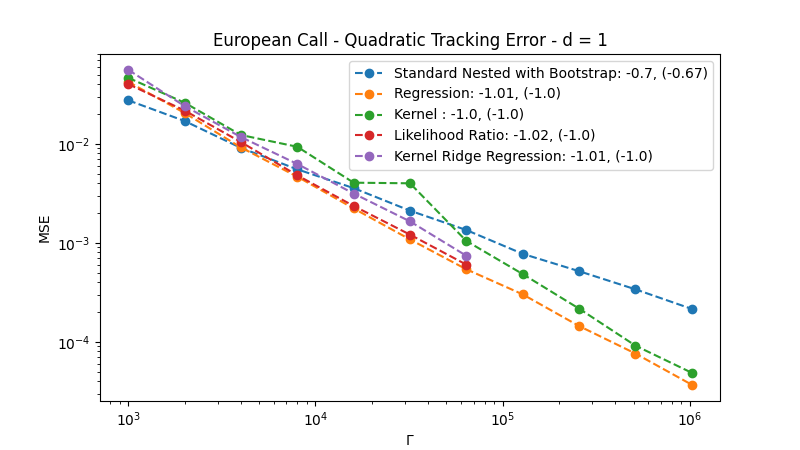
\includegraphics[width=0.7\textwidth]{./project1/figures/figure1.png}
    \caption{Empirical convergence of nested simulation procedures for quadratic tracking error on Portfolio 1 with $d=1$}
    \label{fig1:compareAll} 
\end{figure}
In Figure~\ref{fig1:compareAll}, the MSEs of the nested simulation procedures are plotted against the total simulation budget $\Gamma$ in a log-log scale, where each point represents the average MSE of the corresponding estimator over 1000 replications.
The MSEs of the nested simulation procedures are fitted with a regression line, and the slope of the fitted line is reported as the first number in the legend.
The second number in the legend is the corresponding asymptotic rate of convergence obtained from the theoretical analysis.
The slope of the fitted line can be regarded as the empirical rate of convergence of the corresponding procedure.
By comparing the empirical rates of convergence with the asymptotic rates, we can observe that the empirical rates of convergence of the standard, the kernel smoothing-based, the regression-based, the likelihood ratio-based, and the KRR-based procedures all closely match their asymptotic rates.
Due to the computational complexity of the likelihood ratio-based and the KRR-based procedures, their MSEs are not reported for $\Gamma$ larger than $16,000$ and $64,000$, respectively.
Due to the difficulty of fixing $\Gamma$ for the multi-level Monte Carlo procedure, the empirical rate of convergence of the multi-level Monte Carlo procedure is not reported here, but a detailed analysis of the empirical convergence of the multi-level Monte Carlo procedure is provided in Section~\ref{sec1:empirical-mlmc}.
In the following sections, we examine the empirical convergence of the nested simulation procedures in a similar manner as in Figure~\ref{fig1:compareAll}.
With a more detailed analysis of different risk measures, option types, and asset dimensions, we aim to provide a comprehensive understanding of the convergence behavior of the nested simulation procedures in practice.

\subsection{Sensitivity to the Asset Dimension} \label{sec1:sensitivity-dimension}
In portfolio risk management, the asset dimension is a critical factor that determines the complexity of the portfolio and the computational cost of the risk measure estimation.
The theoretical analyses in Section~\ref{sec1:convergence-orders} suggest that the asymptotic rate of convergence of the nested simulation procedures, except for the kernel smoothing-based procedure, is independent of the asset dimension.
However, the empirical convergence behavior of the nested simulation procedures could be sensitive to the asset dimension.
In this section, we examine the empirical convergence of the nested simulation procedures for different asset dimensions.

\begin{figure}[ht!]
    \centering
    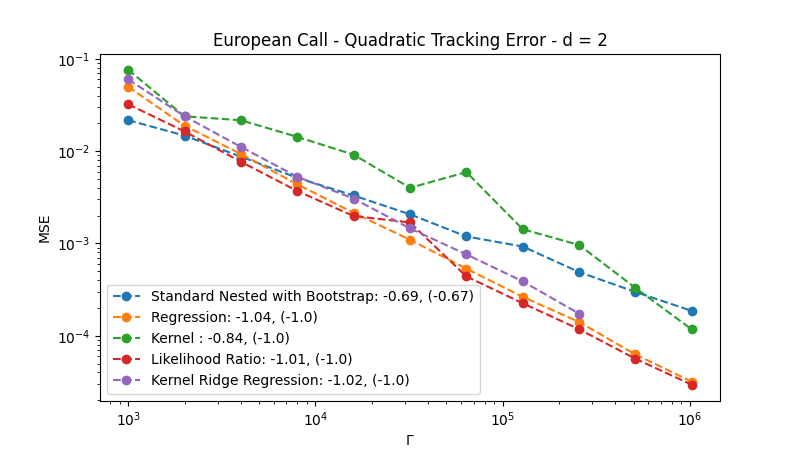
\includegraphics[width=0.48\textwidth]{./project1/figures/figure2a.png}
    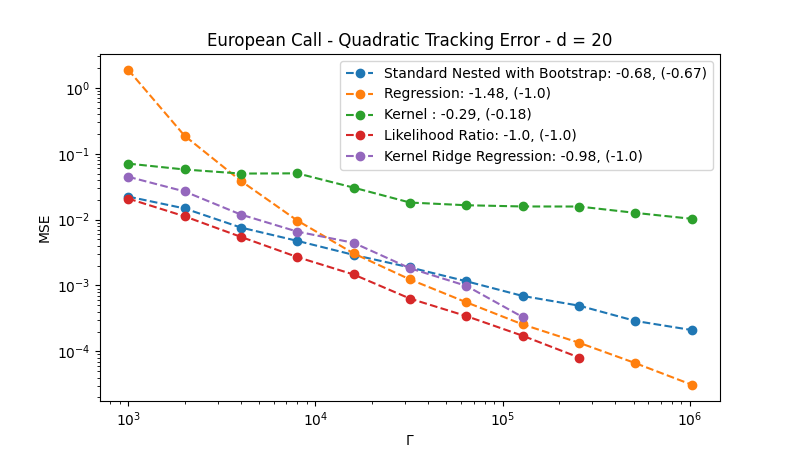
\includegraphics[width=0.48\textwidth]{./project1/figures/figure2b.png}
    \caption{Empirical convergence of nested simulation procedures for quadratic tracking error on Portfolio 1 with different asset dimensions}
    \label{fig1:assetDimension} 
\end{figure}

In Figure~\ref{fig1:assetDimension}, the empirical convergence of the nested simulation procedures for a quadratic tracking error on Portfolio 1 is illustrated for different asset dimensions, i.e., $d = 2$ and $d = 20$.
The empirical rates of convergence of the standard, the KRR-based, and the likelihood ratio-based procedures closely match their asymptotic rates for both asset dimensions, and they are independent of the asset dimension.
On the other hand, the empirical rates of convergence of the kernel smoothing-based and regression-based procedures are higher than their asymptotic rates for both asset dimensions.
They are sensitive to the asset dimension but in different ways.
The empirical rate of convergence of the kernel smoothing-based procedure decreases as the asset dimension increases.
This phenomenon is consistent with the theoretical analysis in Section~\ref{sec1:asymptotic-convergence}, where the asymptotic rate of convergence of the kernel smoothing-based procedure is shown to be sensitive to the asset dimension.
However, the empirical rate is still higher than its asymptotic rate for $d = 2$ and $d = 20$.
The empirical rates of convergence of the regression-based procedure is higher than its asymptotic rates for both asset dimensions, and the empirical rate is higher for $d = 20$ than for $d = 2$.

\subsection{Empirical Convergence of Parametric Regression Procedures} \label{sec1:regression-convergence}

For both the regression-based and the kernel smoothing-based procedures, the reason for the higher empirical rates can be explained by having poor proxy estimators for smaller simulation budgets.
For lower simulation budgets, the proxy estimators of the true inner simulation are poor, and the MSEs of the regression-based and kernel smoothing-based procedures are dominated by the model error of the proxy estimators.
In other words, they have not reached their asymptotic regimes yet.
Due to computation constraints, we are not able to conduct experiments for kernel smoothing-based nested simulation procedures for higher budget levels, but we are able to conduct additional experiments for the regression-based nested simulation procedure.
In our previous numerical experiments, the empirical rate of convergence of the regression procedure is observed to be much larger than its asymptotic rate of convergence.
For dimensions larger than 10, the MSE of the regression procedure decreases quickly in the beginning, and it stabilizes after a certain budget level.
In~\ref{fig1:reg_lb} illustrates the empirical convergence of the regression-based procedure in more detail at higher simulation budgets, where the asymptotic level of convergence is reached for $d = 20$.

\begin{figure}[ht]
    \centering
    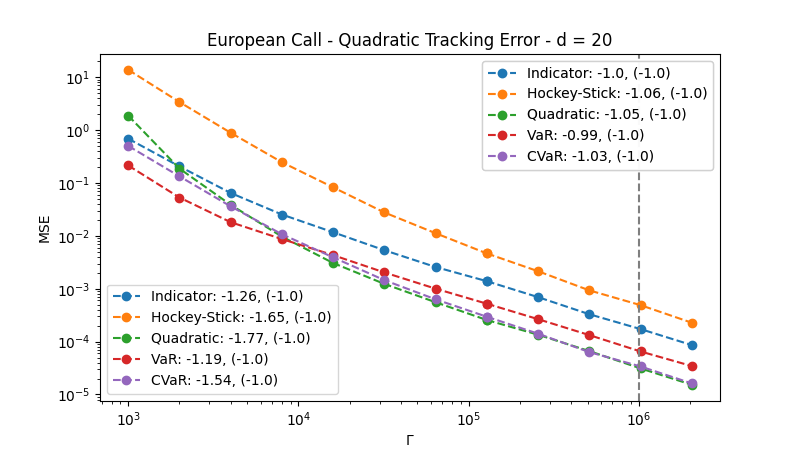
\includegraphics[width=0.7\textwidth]{./project1/figures/figure3.png}
    \caption{Empirical convergence of regression procedure for European call options and $d=20$}
    \label{fig1:reg_lb} 
\end{figure}

The left part of Figure \ref{fig1:reg_lb} contains the MSEs of the regression procedure for budget sizes that are smaller than $10,000$. 
Slopes of the fitted lines on the left correspond to the empirical rate of convergence of the regression procedure for budget levels between $1,000$ and $10,000$.
To investigate the convergence behavior for higher budget levels, we conduct additional experiments for the European call option with dimension $20$. 
The additional experiments are summarized on the right of Figure \ref{fig1:reg_lb}.
After reaching a certain budget level, i.e., $\Gamma = 1,000,000$, the empirical rate of convergence for the regression-based nested simulation procedure approaches its asymptotic rate. 
For nested simulation procedures whose proxy models are biased, the proxy estimators of the true inner simulation are poor, especially for smaller budget sizes. 
We are able to clearly observe this phenomenon for the regression proxy, and it can be explained by dividing the MSE into proxy bias and simulation variance.
For small budget sizes, the improvement of the bias of the regression proxy dominates the improvement of simulation variance. 
Performing poorly for extremely low simulation budgets, the regression proxy improves significantly. 
As the simulation budget gets higher, the improvement of the regression proxy becomes negligible compared with that of the simulation variance. 
The regression proxy ceases to improve after reaching a certain level ($\Gamma = 100\!,\!000$ in our case), and the improvement of simulation variance dominates.

\subsection{Empirical Convergence of Kernel Smoothing-Based Procedures} \label{sec1:kernel-smoothing-convergence}

The kernel smoothing proxy is a nonparametric regression procedure.
According to the theoretical analysis in Section~\ref{sec1:asymptotic-convergence}, the asymptotic rate of convergence of the kernel smoothing-based nested simulation procedure is highly dependent on the dimension of the asset.

\begin{figure}[ht!]
    \centering
    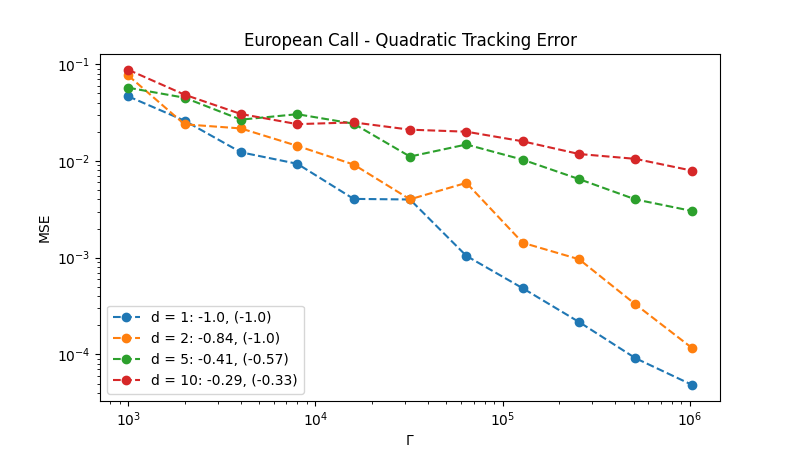
\includegraphics[width=0.48\textwidth]{./project1/figures/figure4a.png}
    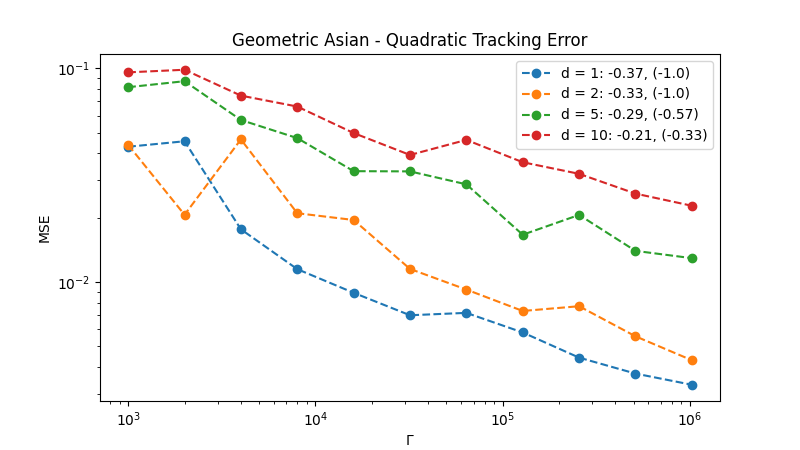
\includegraphics[width=0.48\textwidth]{./project1/figures/figure4b.png}
    \caption{Empirical convergence of kernel smoothing procedure for different values of $d$}
    \label{fig1:kernel_d} 
\end{figure}

In Figure~\ref{fig1:kernel_d}, the empirical convergence of the kernel smoothing-based nested simulation procedure for quadratic tracking error is illustrated for different asset dimensions, i.e., $d = 1, 2, 5, 10$.
The observation finds that the kernel smoothing-based nested simulation procedure is extremely sensitive to the asset dimension and the payoff structure.
While the asset dimension is expected to be a critical factor as shown in the theoretical analysis, the payoff structure is an unexpected factor that affects the empirical convergence of the kernel smoothing-based nested simulation procedure.
For a portfolio with geometric Asian options, the payoff complexity is higher than that of a portfolio with European call options.
The empirical rate of convergence of the kernel smoothing-based procedure is significantly lower for the portfolio with geometric Asian options than for the portfolio with European call options.
For geometric Asian options, the empirical rates of convergence are even lower than the asymptotic rates for all asset dimensions.

Due to the computational cost of the kernel smoothing-based nested simulation procedure, we are not able to conduct experiments for higher budget levels.
However, we are able to conduct additional experiments to examine the effects of cross-validation on the empirical convergence of the kernel smoothing-based procedure.
Another phenomenon that is observed in Figure~\ref{fig1:kernel_d} is that the empirical rate of convergence of the kernel smoothing-based procedure does not decrease monotonically as the simulation budget increases.
This is likely due to the fact that the kernel smoothing-based procedure, as a nonparametric regression procedure, is highly dependent on the cross-validation of the proxy hyperparameters.
For the kernel smoothing-based procedure, the kNN proxy is implemented. 
Hence, the proxy hyperparameter is the number of nearest neighbors $k$.
In our numerical experiment, cross-validation is conducted once to select the optimal value of $k$ for each simulation budget, and the selected value of $k$ is fixed for all $1,000$ replications.
Therefore, a poor selection of the optimal value of $k$ can lead to a poor proxy estimator, and the MSE of the kernel smoothing-based procedure will be dominated by the model error of the proxy estimator.

\begin{figure}[ht!]
    \centering
    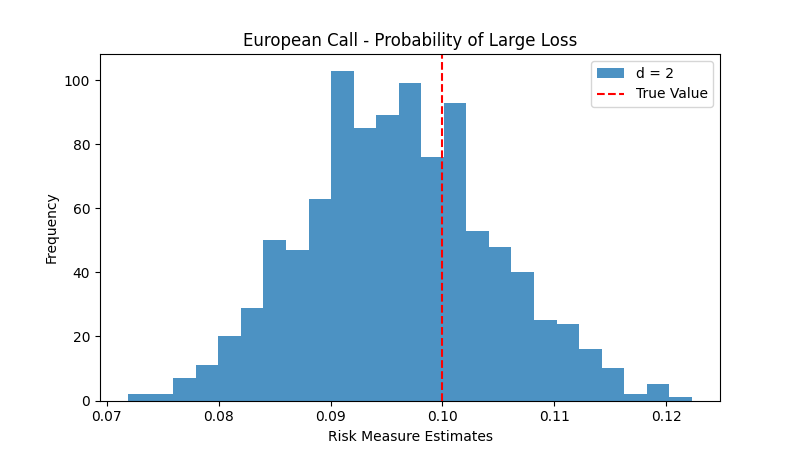
\includegraphics[width=0.48\textwidth]{./project1/figures/figure5a.png}
    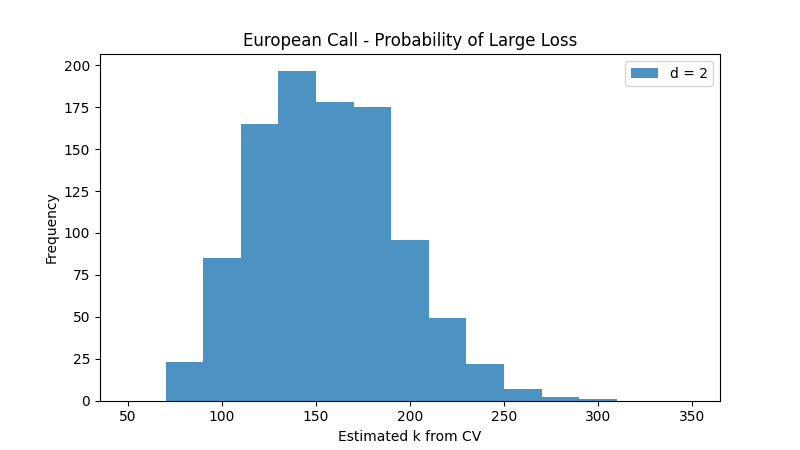
\includegraphics[width=0.48\textwidth]{./project1/figures/figure5b.png}
    \caption{Cross-validation for the kernel smoothing-based procedure with $\Gamma=100,000$}
    \label{fig1:kernel_cv} 
\end{figure}

In Figure~\ref{fig1:kernel_cv}, the empirical convergence of the kernel smoothing-based nested simulation procedure for the probability of large loss is illustrated for different values of $k$ with $\Gamma = 100,000$.
The observation is that the value of optimal $k$ estimated by cross-validation is highly variable across different replications.
For the two replications where $k = 80$ is selected as the optimal value of $k$, the estimated risk measures for the kernel smoothing-based procedure are $0.1187$ and $0.1189$, which are significantly higher than the estimated risk measures for the other replications and far from the true risk measure of $0.1$.
This observation suggests that the empirical convergence of the kernel smoothing-based nested simulation procedure is highly dependent on the cross-validation of the proxy hyperparameters.

\subsection{Sensitivity to the Option Types and Risk Measures} \label{sec1:sensitivity-option-type}

In our previous numerical experiments, we have examined the empirical convergence behavior of the nested simulation procedures for European call options, which is the most basic option type.
To examine the sensitivity of the empirical convergence behavior to the option type, we consider path-dependent options, namely geometric Asian options and barrier options.

\begin{figure}[ht!] 
    \centering
    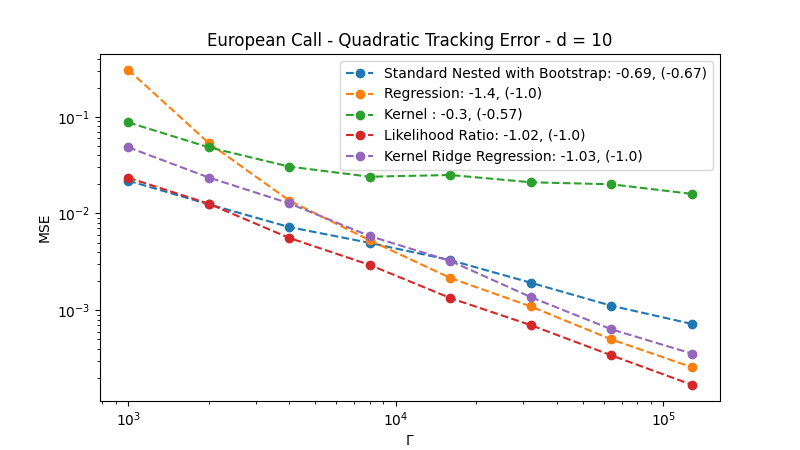
\includegraphics[width=0.48\textwidth]{./project1/figures/figure6a.png}
    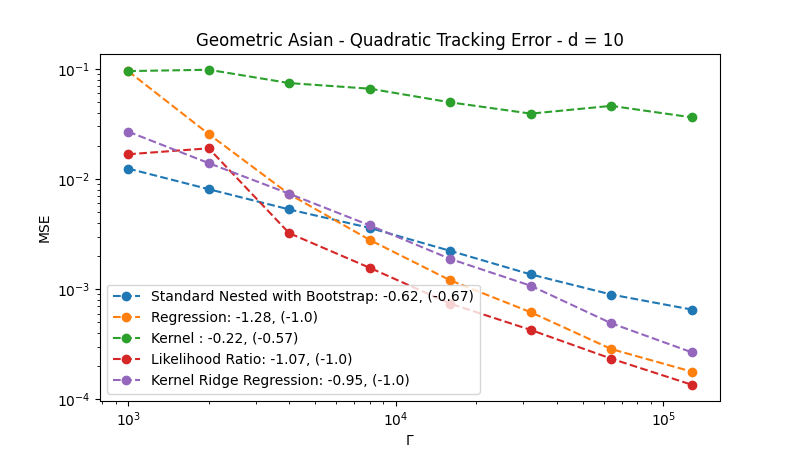
\includegraphics[width=0.48\textwidth]{./project1/figures/figure6b.png}
    \caption{Empirical convergence of nested simulation procedures for quadratic tracking error on different portfolios with $d=20$}
    \label{fig1:1x03} 
\end{figure}

In Figure~\ref{fig1:1x03}, the empirical convergence of the nested simulation procedures for the quadratic tracking errors of Portfolio 1 and Portfolio 4 is illustrated for $d = 20$.
The empirical rates of standard, likelihood ratio-based, and KRR-based nested simulation procedures closely ensemble their asymptotic rates for path-dependent options.
The empirical rate of convergence of the regression-based and kernel smoothing-based procedures is much higher than their asymptotic rates for barrier options, with reasons explained in Section~\ref{sec1:regression-convergence}.

\begin{figure}[ht!] 
    \centering
    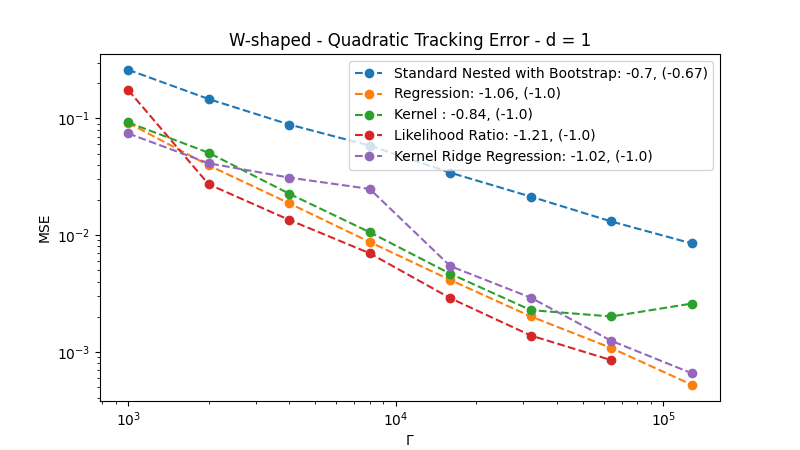
\includegraphics[width=0.48\textwidth]{./project1/figures/figure7a.png}
    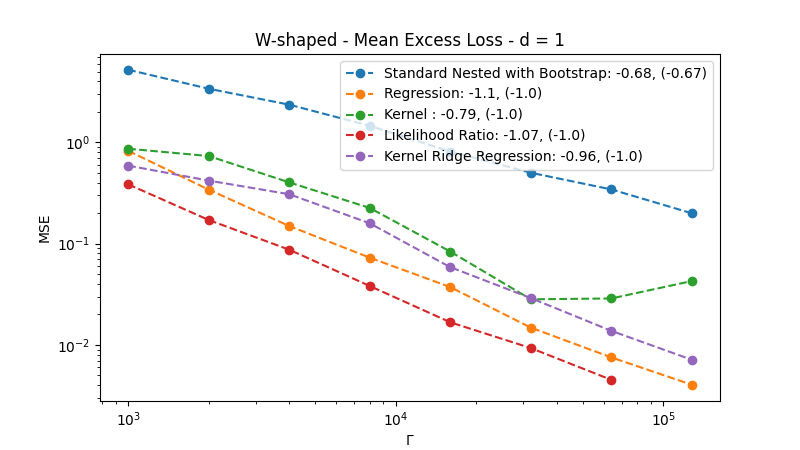
\includegraphics[width=0.48\textwidth]{./project1/figures/figure7b.png}
    \caption{Empirical convergence of nested simulation procedures for a W-shaped payoff}
    \label{fig1:5503} 
\end{figure}

In~\cite{broadie2015risk}, the authors propose a numerical example where the payoff has a W-shape with respect to the underlying asset price.
We have incorporated this example as Portfolio 5.
In Figure~\ref{fig1:5503}, the empirical convergence of the nested simulation procedures for quadratic tracking error and mean excess loss on Portfolio 5 is illustrated for $d = 1$.
For all procedures, we observe a similar convergence behavior as in other path-dependent options.
The MSEs of the kernel smoothing-based and KRR-based procedures do not decrease monotonically as the simulation budget increases, as observed and analyzed in Section~\ref{sec1:kernel-smoothing-convergence}.

\begin{figure}[ht!] 
    \centering
    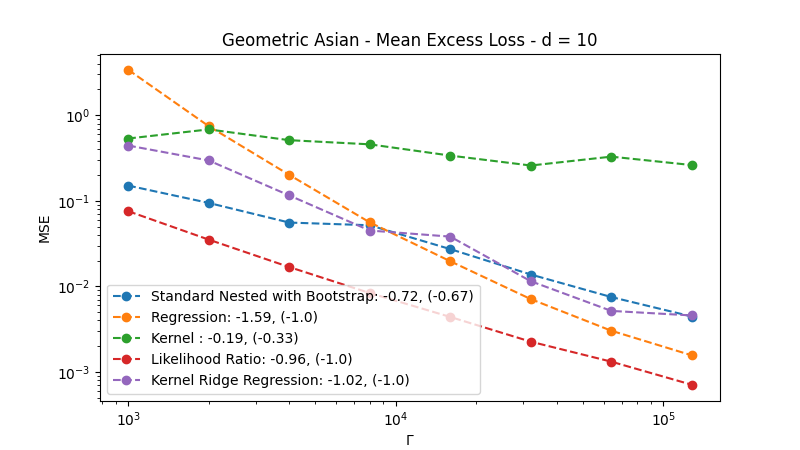
\includegraphics[width=0.48\textwidth]{./project1/figures/figure8a.png}
    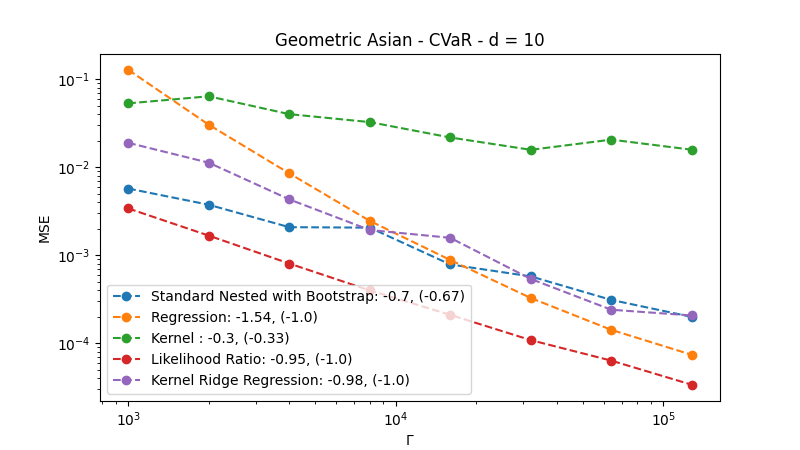
\includegraphics[width=0.48\textwidth]{./project1/figures/figure8b.png}
    \caption{Empirical convergence of nested simulation procedures for different risk measures on Portfolio 1 with $d=20$}
    \label{fig1:110x}
\end{figure}

Figure~\ref{fig1:110x} illustrates similar observations for sensitivity to different risk measures.
A change in the risk measure of interest does not affect the empirical convergence behavior of all nested simulation procedures.
From the empirical convergence results, we observe that the empirical rates of convergence of the regression-based nested simulation procedure are the highest among all nested simulation procedures for all risk measures and option types.
Furthermore, the regression-based procedure is stable across different payoff structures and risk measures. 
Its MSEs decrease quickly in the beginning, and after reaching a certain budget level, the rate of decrease stabilizes to match its asymptotic rate of convergence.

\subsection{Sensitivity to level for VaR and CVaR} \label{sec1:sensitivity-level}

The level of VaR and CVaR is a critical factor that determines the complexity of the risk measure estimation.
In our previous numerical experiments, the level of VaR and CVaR is set to be the 90\% quantile of the distribution of the inner simulation noise.
In this section, we examine the empirical convergence of the regression-based nested simulation procedures for different levels of VaR and CVaR, i.e., $80\%$, $90\%$, $95\%$, $99\%$, and $99.6\%$.

\begin{figure}[ht!] 
    \centering
    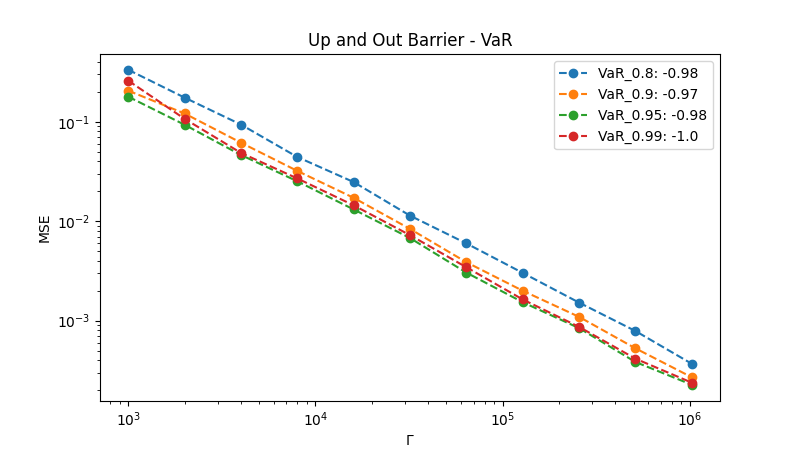
\includegraphics[width=0.48\textwidth]{./project1/figures/figure9a.png}
    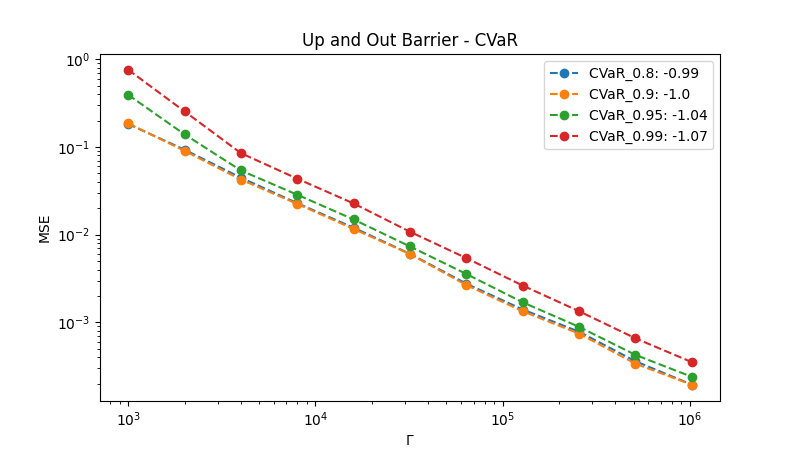
\includegraphics[width=0.48\textwidth]{./project1/figures/figure9b.png}
    \caption{Empirical convergence of regression-based procedures for different levels of VaR and CVaR for Up and Out Barrier Call Options}
    \label{fig1:sens_level}
\end{figure}

In Figure~\ref{fig1:sens_level}, the empirical convergence of the regression-based nested simulation procedure for different levels of VaR and CVaR is illustrated for up-and-out barrier call options.
The empirical rates of convergence of the regression-based nested simulation procedure are independent of the level of VaR and CVaR.

\subsection{Sensitivity to the Asset Model} \label{sec1:sensitivity-assetModel}

Our previous numerical experiments have been conducted under the assumption that the underlying asset dynamics follow a multidimensional geometric Brownian motion with $0.3$ pairwise correlation.
To examine the sensitivity of the empirical convergence behavior to the asset model, we consider a stochastic volatility model, i.e., a Heston model.

\begin{figure}[ht!] 
    \centering
    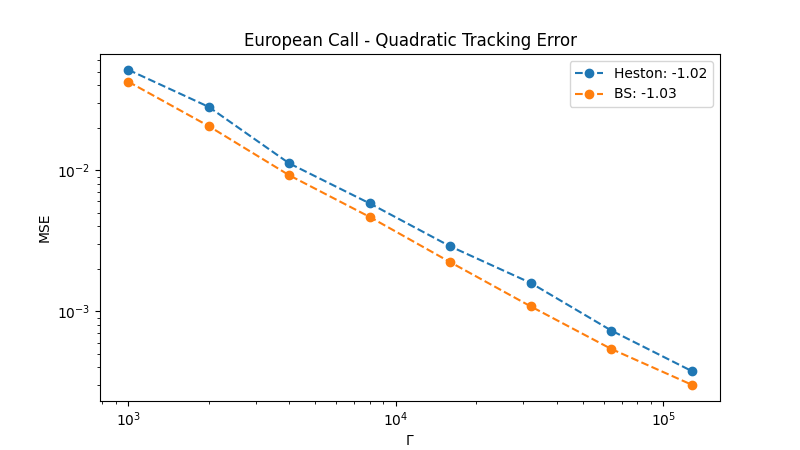
\includegraphics[width=0.48\textwidth]{./project1/figures/figure10a.png}
    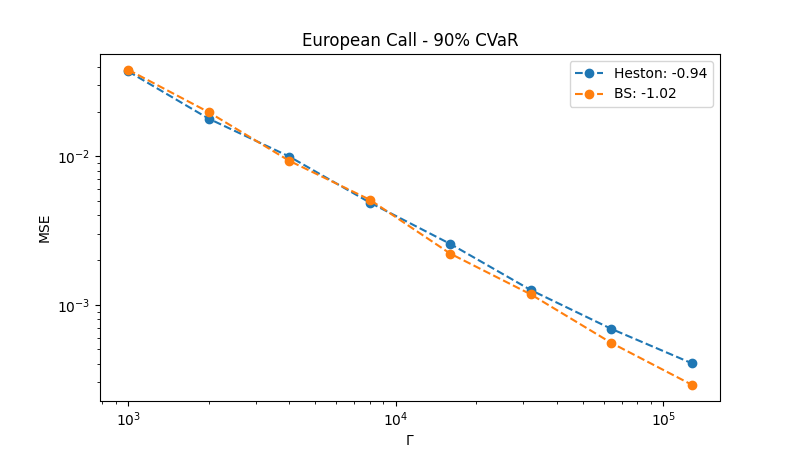
\includegraphics[width=0.48\textwidth]{./project1/figures/figure10b.png}
    \caption{Empirical convergence of regression-based nested simulation procedures for different asset models}
    \label{fig1:sens_model}
\end{figure}

In Figure~\ref{fig1:sens_model}, the empirical convergence results of the regression-based nested simulation procedure for a quadratic tracking error and a 90\%-CVaR are illustrated for different asset models, i.e., a geometric Brownian motion and a Heston model.
The empirical rates of convergence of the regression-based nested simulation procedure are observed to be independent of the asset model.

\subsection{Empirical Convergence of Multi-level Monte Carlo} \label{sec1:empirical-mlmc}

The multi-level Monte Carlo procedure is a variance reduction technique that is designed to reduce the computational cost of nested simulation procedures.
The theoretical analysis in~\cite{giles2019multilevel} shows that the multi-level Monte Carlo procedure has a faster empirical rate of convergence than the standard nested simulation procedure when the risk measure of interest is the probability of a large loss over a threshold $u$, i.e., the nested expectation case with $h$ being an indicator function.

\begin{table}[ht]
    \centering
    \begin{tabular}{rrrrrr}
    \toprule
    \textbf{Level} & \textbf{Bias} & \textbf{Variance} & \textbf{MSE} & $\Gamma$ & \textbf{MSE of SNS} \\ 
    \hline\hline
    0 & 0.118  & 0.104  & 0.1364 & 6400     & 0.1660    \\
    1 & 0.102  & 0.0916 & 0.1020 & 27600    & 0.1305    \\
    2 & 0.0870 & 0.0794 & 0.0870 & 76600    & 0.0954    \\
    3 & 0.0815 & 0.0746 & 0.0812 & 175600   & 0.0744    \\
    4 & 0.0893 & 0.0805 & 0.0884 & 348100   & 0.0460    \\
    5 & 0.0750 & 0.0694 & 0.0750 & 640000   & 0.0366    \\
    \bottomrule
    \end{tabular}
    \caption{MSEs of the multi-level Monte Carlo procedure for different levels}
    \label{tab1:mlmc-mse}
\end{table}

Instead of using a figure, we provide a summary of the empirical convergence results of the multi-level Monte Carlo procedure with a decomposition table of the MSEs in Table~\ref{tab1:mlmc-mse}.
The MSEs of the multi-level Monte Carlo procedure are decomposed into the bias and the variance of the estimator.
The MSEs of the standard nested simulation procedure with a similar total simulation budget are also provided for comparison.
Since the multi-level Monte Carlo procedure is designed with a fixed number of outer simulation paths, the benefit of the multi-level Monte Carlo procedure is minimal when the total simulation budget is large.
More specifically, when $\Gamma$ is large, the standard nested simulation procedure with a bootstrap-based budget allocation strategy benefits from having a larger number of outer simulation paths, and the MSE of the standard nested simulation procedure is lower than that of the multi-level Monte Carlo procedure with a fixed number of outer simulation paths.


\section{Computational Complexity} \label{sec1:computational-complexity}
Compared to the standard procedure, proxy-based nested simulation procedures often have faster empirical rates of convergence.
The faster convergence benefits from the pooling of inner samples through the proxy models. 
However, pooling itself comes with computational costs, which are usually ignored in most numerical comparisons. 
This section summarizes the algorithmic complexity and illustrate the computational time of different nested simulation procedures.
The findings can provide some further guidance on the choice of a proper nested simulation procedure given a nested estimation problem.
Define basic operations to be basic mathematical operators, that is, arithmetic with individual elements has complexity $\mathcal{O}(1)$.

\begin{table}[ht]
    \centering  
    \small
    \begin{tabular}{llll}
    \hline
    \textbf{Procedures}      & \textbf{Training cost}                    &  \textbf{Prediction cost}    & \textbf{Total additional cost} \\ \hline \hline
    Standard procedure       &  $0$                                      &  $\mathcal{O}(M)$            & $\mathcal{O}(M)$ \\ 
    Regression               &  $\mathcal{O}(p^2M) + \mathcal{O}(p^3)$   &  $\mathcal{O}(pM)$           & $\mathcal{O}(p^2M) + \mathcal{O}(p^3)$ \\
    Kernel smoothing         &  $\mathcal{O}(M\log(M))$                  &  $\mathcal{O}(k\log(M))$     & $\mathcal{O}(M\log(M))$ \\
    Kernel ridge regression  &  $\mathcal{O}(M^3)$                       &  $\mathcal{O}(M^2)$          & $\mathcal{O}(M^3)$ \\
    Likelihood ratio         &  $0$                                      &  $\mathcal{O}(M^2)$          & $\mathcal{O}(M^2)$ \\
    \hline
    \end{tabular} 
    \caption{Additional computational costs of nested simulation procedures aside from simulation}
    \label{tab1:complexity}
\end{table}

Table~\ref{tab1:complexity} shows the algorithmic complexity of the nested simulation procedures.
For a $d$-dimensional nested estimation problem, the simulation cost for all procedures is $\mathcal{O}(dMN)$.
The simulation cost is omitted from Table~\ref{tab1:complexity}, as all methods are given the same simulation budget.
Given $M$ outer samples and the corresponding $M$ inner sample averages, the algorithmic complexity of the additional operations does not involve $N$ thus can be written in terms of $M$ only.
The training cost includes the cost of fitting the proxy model and the cost of cross-validation for nonparametric regression proxies.
For the standard procedure, the training cost is $0$ due to the absence of proxy models. 
Its prediction cost $\mathcal{O}(M)$ comes from the evaluation of the function $h$ for $M$ samples.
For the regression-based procedure, a linear regression model is fitted with $p$ predictors.
In practice, $p$ is usually much smaller than $M$ and does not grow with the simulation budget $\Gamma$.
However, it is dependent on the complexity of the payoff function.
Estimating the coefficients of the regression model involves multiplying the design matrix by its transpose and inverting the resulting matrix, which has complexity $\mathcal{O}(p^2M)$ and $\mathcal{O}(p^3)$, respectively.
For a review in the complexity of matrix inversion, see~\cite{stothers2010complexity}.
The matrix inversion has complexity $\mathcal{O}(p^3)$ using Gauss-Jordan elimination, but in practice, the complexity can be reduced to $\mathcal{O}(p^{2.807})$ by~\cite{strassen1969gaussian} and $\mathcal{O}(p^{2.376})$ by~\cite{coppersmith1987matrix}.
The prediction cost of the regression-based procedure is $\mathcal{O}(pM)$, which comes from the multiplication of the design matrix by the estimated coefficients.
For the kernel smoothing-based procedure, the kNN proxy is implemented.
In practice, the K-D tree algorithm~\citep{bentley1975multidimensional} is often implemented for efficient nearest neighbor search.
During training, a tree is constructed to store the distance, which has complexity $\mathcal{O}(M\log(M))$.
The prediction cost of the kernel smoothing-based procedure is $\mathcal{O}(kM\log(M))$, which comes from a query of the K-D tree for $k$ nearest neighbors for $M$ samples.
Conversely, An inefficient algorithm calculates the distance matrix during training and a block sort algorithm to find the $k$ nearest neighbors, which results in a complexity of $\mathcal{O}(M^2)$ and $\mathcal{O}(M^2\log(M))$, respectively.
A practical implementation of block sort is provided in~\cite{kim2008ratio}.
Hence, an efficient implementation of the kNN proxy is crucial for the kernel smoothing-based procedure.
For the likelihood ratio-based procedure, the training cost is $0$ as no training is required.
The prediction cost of the likelihood ratio-based procedure is $\mathcal{O}(M^2)$, which comes from the calculation of the likelihood weights for $M$ samples.
For the KRR-based procedure, the main training cost comes from inverting an $M \times M$ kernel matrix~\citep{scholkopf2002learning}, which has complexity $\mathcal{O}(M^3)$ using Gauss-Jordan elimination.
Similar to the regression-based procedure, this complexity can be reduced to $\mathcal{O}(M^{2.376})$.
The prediction cost of the KRR-based procedure is $\mathcal{O}(M^2)$, which comes from the multiplication of the kernel matrix by the estimated coefficients.
Among the proxy-based procedures, regression is the most efficient as $p$ is usually much smaller than $M$. 
Kernel smoothing and KRR are kernel-based proxies, and they are more expensive due to distance calculation and cross-validation of hyperparameters. 
The kNN proxy has only 1 hyperparameter $k$, while the KRR proxy requires 3 hyperparameters, namely the smoothness hyperparameter $\nu$, scale hyperparameter $\upsilon$, and the regularization hyperparameter $\lambda$.
Calculating the likelihood ratio weights is inevitable for the likelihood ratio-based procedure. 
While a k-fold cross-validation is used to estimate the hyperparameter for kNN, the KRR requires Bayesian optimization~\citep{shahriari2015taking} to estimate the hyperparameters due to having a high-dimensional search space.
The likelihood ratio-based procedure requires no training, but the cost of calculating the likelihood weights is $\mathcal{O}(M^2)$.
Comparing the algorithmic complexity of the nested simulation procedures, the regression-based procedure is the most efficient among the proxy-based procedures.
For a fixed $p$, the total additional cost of a regression-based procedure is $\mathcal{O}(M)$, which is the same as the standard procedure's.


\begin{figure}[ht!]
    \centering
    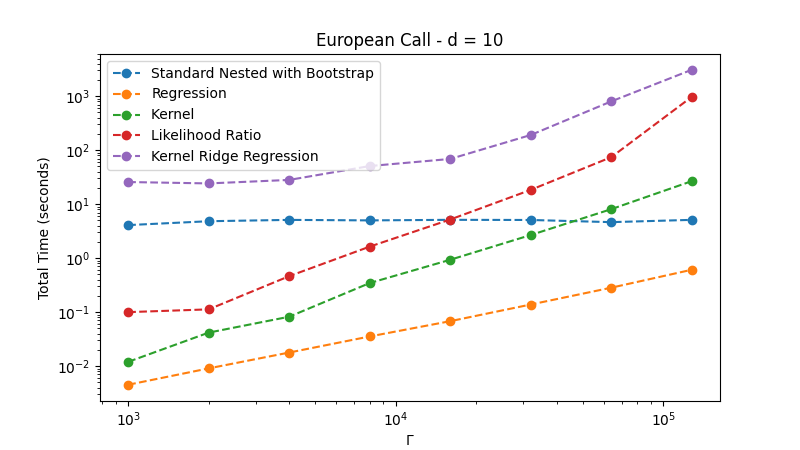
\includegraphics[width=0.48\textwidth]{./project1/figures/figure11a.png}
    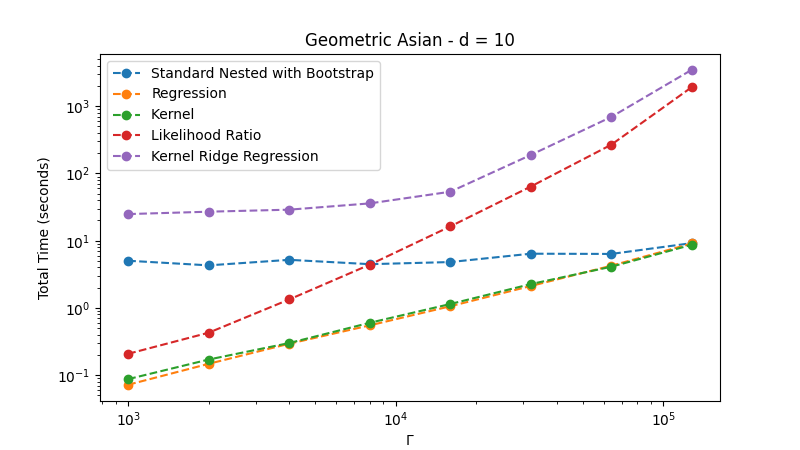
\includegraphics[width=0.48\textwidth]{./project1/figures/figure11b.png}
    \caption{Total computational cost for different procedures with $d=10$}
    \label{fig1:tcc}
\end{figure}

In our finite-sample experiments, we have observed that the actual computational cost to be significantly different from the theoretical complexity, as not only the order of complexity but also the constant factors can affect the computational cost.
In Figure~\ref{fig1:tcc}, the total computational time of different nested simulation procedures for European call options and geometric Asian options with $d = 10$ is illustrated in a log-log scale.
The $x$-axis shows the total simulation budget $\Gamma$, and the $y$-axis is the total computational time for 1 replication of the numerical experiment, in seconds.
All procedures are implemented on a machine with an AMD Ryzen 9 7900X processor with 32GB of RAM.
8 cores are used for parallel computing, and the total computational time is the sum of the simulation time, the training time, and the prediction time.
The regression and kernel smoothing-based procedures are the most efficient among the proxy-based procedures.
Since the regression-based procedure has a higher empirical rate of convergence, it is preferred over the kNN.
The likelihood ratio-based and KRR-based procedures are the most computationally expensive among all procedures.
They are demanding in terms of memory.
For budgets larger than $10^5$, the likelihood ratio-based procedure becomes impractical as storage of the likelihood weights becomes a bottleneck.
The KRR-based procedure suffers from both cross-validation and inverting a kernel matrix of size $M \times M$.
To separate the total computational time into different attributes, we provide a detailed analysis of the total computational time in the remainder of this section.

\begin{figure}[ht!]
    \centering
    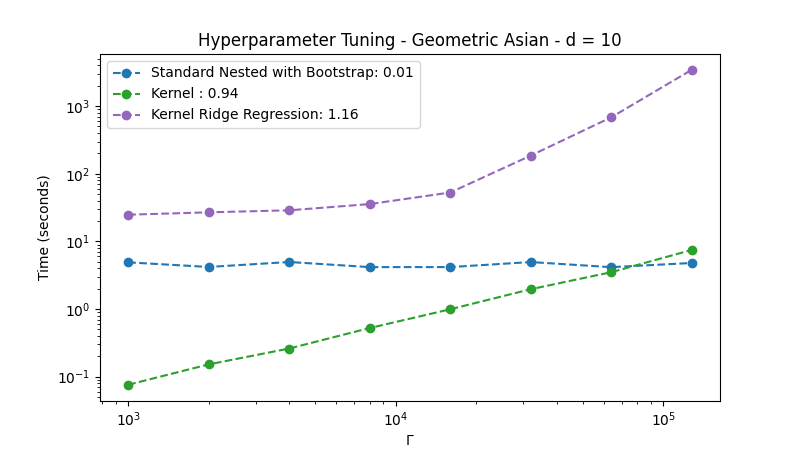
\includegraphics[width=0.48\textwidth]{./project1/figures/figure12a.png}
    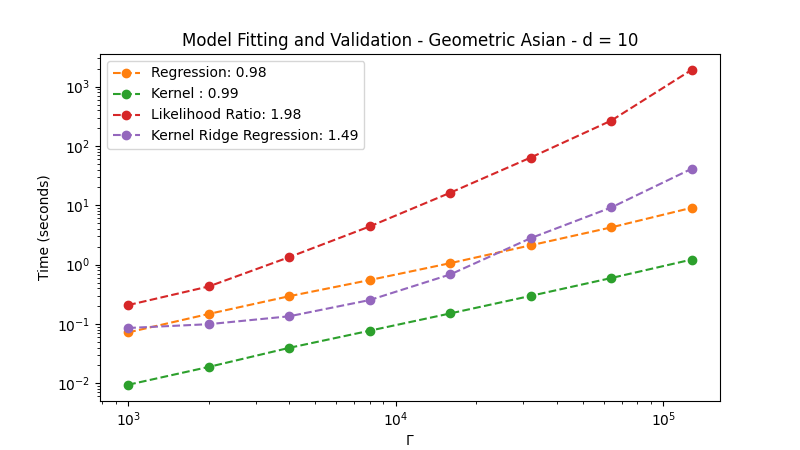
\includegraphics[width=0.48\textwidth]{./project1/figures/figure12b.png}
    \caption{Computational cost for implementing nested simulation procedures with $d=10$, excluding simulation time}
    \label{fig1:c_model}
\end{figure}

Figure~\ref{fig1:c_model} illustrates the computational time of implementing different nested simulation procedures for the portfolio of geometric Asian options with $d = 10$, excluding the simulation time.
The simulation time is omitted as it is the same for all procedures.
The remainder can be decomposed into two parts: hyperparameter tuning and model implementation.
The hyperparameter tuning cost is the cost of estimating the optimal hyperparameters for the proxy models, and the model implementation cost is the cost of fitting the proxy models and generating predictions from the trained proxies.
For each procedure, each point in Figure~\ref{fig1:c_model} represents the average computational time for a given simulation budget $\Gamma$.
A regression model is fitted to each model respectively, and its slope is reported as the growth rate of the computational time with respect to $\Gamma$.
The total computational time of the standard procedure is mostly attributed to finding the optimal $M$ and $N$ using the bootstrap-based budget allocation strategy from~\cite{zhang2021bootstrap}.
This cost does not grow with the simulation budget $\Gamma$, as its slope is close to $0$.
The regression-based procedure does not require hyperparameter tuning, and its total computational time is mainly attributed to the model implementation.
The slope of the regression line is close to $1$, resembling the its algorithmic complexity in Table~\ref{tab1:complexity}.
The kernel smoothing-based and KRR-based procedure requires cross-validation to estimate the optimal hyperparameters.
In our implementaion of kNN, the cross-validation is conducted using a grid search with a search space whose cardinality does not grow with the simulation budget $\Gamma$.
However, the cross-validation cost of the kernel smoothing-based procedure grows with the simulation budget $\Gamma$ as more samples are involved.
The KRR-based procedure requires Bayesian optimization to estimate the optimal hyperparameters, and the cardinality of the search space grows with the simulation budget $\Gamma$.
The empirical cost of the KRR-based procedure does not resemble its algorithmic complexity in Table~\ref{tab1:complexity}.
The efficient implementation of KRR is an active area of research, and the computational cost of KRR can be reduced by using a low-rank approximation of the kernel matrix, e.g., the Nystr\"om method~\citep{nystrom1930praktische}.
Our observation for KRR implementation time is in line with the findings in~\cite{scikit-learn}, where the cost of KRR is reported quickly increasing with the number of samples.
The likelihood ratio-based procedure requires no hyperparameter tuning, and its total computational time is mainly attributed to the likelihood weight calculation, which is $\mathcal{O}(M^2)$. 
In summary, for a large simulation budget, the regression-based procedure is the most efficient among all proxy-based procedures in terms of computational time.

\section{Conclusion} \label{sec1:conclusion}
In the task of estimating risk measures for portfolios of complex financial derivatives, nested simulation procedures are commonly required but often computationally expensive. 
Tremendous efforts have been made to improve the efficiency of nested simulation procedures by approximating the inner simulation model with a proxy model. 
In this study, we review the literature on nested simulation procedures in financial engineering and establish fair comparisons of different proxy models using the same set of numerical examples. 
Asymptotic properties of estimators for different nested simulation procedures are influenced by their corresponding proxy models.
To show an asymptotic convergence result, a more complex proxy model requires a more stringent set of assumptions on the distribution of the outer scenario and the inner simulation noise.
With extensive numerical experiments, we have found the finite-sample performance of a procedure can deviate from its theory. 
In theory, supervised learning-based nested simulation procedures often provide higher rates of convergence, but they come at the computational expense of model training and generating predictions from the trained models. 
The likelihood ratio-based procedure requires no training, but it is computationally expensive to compute and store the likelihood weights.
As a result, the total computational budget is not necessarily the same as the simulation budget, which is usually a limiting factor for practical applications.
A kernel-based procedure, e.g., kNN and KRR, requires cross-validation, and its empirical performance depends heavily the choice of hyperparameters.
A kNN-based procedure is sensitive to the asset dimension and the problem complexity.
A KRR-based procedure is computationally expensive, and its cost grows quickly with the simulation budget.
For kernel-based procedures, the computational cost is heavily dependent on the efficient implementation of the associated algorithms.
For a nested estimation problem with a given computational budget, we suggest the use of the regression-based simulation procedure when the budget size is moderate. 
It is efficient to implement, and it exhibits fast empirical convergence in estimating risk measures for option portfolios. 
However, we have only examined the performance for option portfolios in this study, where finding a suitable set of basis functions for regression is relatively easy.
For payoff functions with high complexity or high dimensionality, the regression-based procedure may not be the best choice.
In practice, a variable annuity contract is often high-dimensional in time with a complex payoff structure, and it is a challenging problem for nested simulation procedures.
In such cases, a neural network-based procedure may be more suitable, as it is a data-driven algorithm that finds a suitable set of basis functions automatically.
In Chapter~\ref{ch2}, we will examine the performance of regression-based and neural network-based nested simulation procedures for estimating risk measures for variable annuities.
